\documentclass[11pt]{article}

\usepackage[hangul]{kotex}
\usepackage{ulem}
\usepackage{romannum}
\usepackage{subfig}
\usepackage{graphicx}
\usepackage[pdfencoding=auto, pdftex]{hyperref}
\input glyphtounicode \pdfgentounicode=1

\graphicspath{{Figs/}}

%%%%%%%%%%

\title{대형 GEM 포일의 품질검증법 및 배송을 위한 포장법에 관한  매뉴얼}
\author{윤인석}
\date{2018년 10월 8일}

%%%%%%%%%%

\begin{document}

\maketitle
\tableofcontents
\listoffigures
\listoftables

\pagenumbering{arabic}

\section{본 문서의 목적}
본 문서의 목적은 메카로에서 생산된 대형 GEM 포일에 대한 올바른 품질검증법과 포장법을 정립하는 것이다. 두 번의 시험 생산\footnote{2017년 12월 2일, 14장의 GE1/1 포일이 배송. 2018년 1월 29일 9장의 GE1/1 포일이 배송.}의 결과 메카로에서 생산된 대형 GEM 포일의 성능 자체는 CERN에서 생산된 대형 GEM 포일과 비슷한 수준으로 측정되었다. 그러나 포일 세척에 미진한 부분이 있는 것으로 파악되고 있다.

대부분의 메카로에서 생산된 GEM 포일은 CERN에서 진행된 품질검증 시험에서 실패했으며, 이 포일을 이용해 조립한 검출기는 작동 중 포일 단락이 일어나 작동이 중지되었다. 반면  Rui 연구실에서 다시 세척한 메카로 GEM 포일은 정상적으로 품질검증 시험에 통과하였다. 그리고 이 재세척된 포일로 조립한 검출기는 가혹한 환경에서 장기간 작동하였음에도 문제 없이 작동하고 있다. 따라서 메카로 GEM 포일은 세척과 배송 중 오염 방지 문제를 제외하면 문제가 없는 것으로 판단된다.

따라서 메카로 GEM 포일의 세척 상태를 검증할 품질검증법을 정립 및 적용하여 포일의 상태를 검증할 필요가 있다. \uline{저품질의 포일이 CERN으로 배송될 경우 Rui 연구실에서 세척 과정을 진행되야 하며, 이 때 상당한 시간적 및 금전적 손해가 발생할 것으로 예상된다. 이는 CMS Phase \Romannum{2} upgrade 프로젝트의 원활한 진행을 방해할 것이며, KCMS에 추가적인 금전적 손해를 강요할 것이다.} 따라서 포일 배송 전 GEM 포일의 품질을 최대한 검증하여 이와 같은 일의 발생을 최소화해야 한다. 또한 포일 포장법을 정립하여 포일이 배송 중 오염되거나 파손되는 일을 최대한 줄여야 한다.

이에 메카로에 파견된 KCMS 구성원이 GEM 포일에 대한 엄격한 품질검증을 진행하고, 올바르게 GEM 포일을 포장하도록 할 것이다. 이는 메카로가 GEM 포일 생산에만 집중할 수 있도록 배려함을 위함이다. 또한 생산과 품질검증을 분리하여 품질검증의 기준이 인적 요소에 의해 낮아지는 것을 방지하기 위함이다. 이에 본 문서는 메카로에 파견된 KCMS 구성원이 진행해야할 품질검증법과 포장법을 안내하는 것을 목적으로 한다.

\section{품질검증법}
품질검증에 실패한 GEM 포일은 포일의 상태에 따라 \uline{인수거부 또는 재세척 의뢰}를 해야한다. \uline{재세척을 한 포일은 품질검증의 처음으로 돌아가 모든 과정을 다시 밟아야 한다.} 

\subsection{광학적 검증법}
광학적 검증법의 목표는 형태에 이상이 있는 GEM 포일을 제거하는 것이다. 형태에 이상이 있는 포일은 되돌리기 매우 어렵기 때문에 문제가 있는 포일은 인수거부 되어야 한다.

\subsubsection{육안검사}
품질검증의 시작은 육안으로 GEM 포일의 형태를 확인하는 외관 검사와, 필름 판독기를 이용한 식각 결합 검사이다. 
\begin{itemize}
\item 외관 검사 : 가장 먼저 HV 패드에 발려있는 은 페이스트가 완전히 건조 되었는지 확인한다. 그림 \ref{fig:undried_paste}은 은 페이스트가 완전히 건조되지 않은 상태에서 포장을 진행하였기 때문에 발생한 현상이다. 은 페이스트가 주변으로 밀려 들어간 것을 확인할 수 있다. 밀려 들어간 은 페이스트가 GEM 포일의 활성 영역으로 들어가면, 포일이 단락되며, 이를 복구할 수 없다.\\
  그림 \ref{fig:example_damaged_foils}처럼 공정 과정 상 어쩔 수 없이 발생하는 작은 구겨짐 외에 찍힘, 또는 접힘 등의 물리적 손상이 보일 경우, 포일의 장기간 안정성을 보장할 수 없다. 따라서 \uline{해당 포일을 인수 거부해야 한다.}\\
  이 외에도 SMD 저항이 빠짐 없이 그리고 정상적인 위치에 납땜이 되어 있는지 확인해야 한다. 또한 HV 라인에 끊어진 곳이 없이 정상적으로 형성이 되어 있는지도 확인해야 한다.
\item 식각 결함 검사 : 외관 검사를 통과한 포일은 식각 결함의 정도를 확인하기 위하여 그림 \ref{fig:light_board}처럼 필름 판독기에 포일을 올려 놓는다. 식각 결함이 있는 부분은 다른 곳보다 밝게 보이므로 이를 통해 결함이 있는 위치를 확인할 수 있다. 그림 \ref{fig:example_defect}은 식각 결함의 예를 보여준다.\\
  그림 \ref{fig:example_defect}의 왼쪽 사진처럼 구리층만 손상되었을 경우 대체로 큰 문제는 없다. 단지 해당하는 활성 영역을 잃을 뿐이고, 검출기를 운영하는데 그외의 문제가 발생하지 않기 때문이다. 정해진 기준은 없으나, 결함 면적이 5 mm$^2$ 이하라면 충분히 감수가능하다고 생각된다. 대체로 메카로 GEM 포일은 CERN에서 생산한 GEM 포일에 비해 이런 종류의 결함이 적은 것으로 관찰되었기 때문에 PI층이 온전한 결함의 경우 큰 신경을 쓰지 않아도 무방하다.\\
  그러나 \uline{그림 \ref{fig:example_defect}의 오른쪽 사진처럼 PI층까지 손상을 입었을 경우 이는 매우 중대한 결함을 의미 할 수 있으므로 반드시 현미경을 통해 손상 양상을 확인해야 한다. 특히 결함이 포일이 구겨진 위치에 존재한다면, 해당 포일은 매우 신중하게 검사를 진행해야 한다.}
\end{itemize}

\begin{figure}[htb]
  \centering
  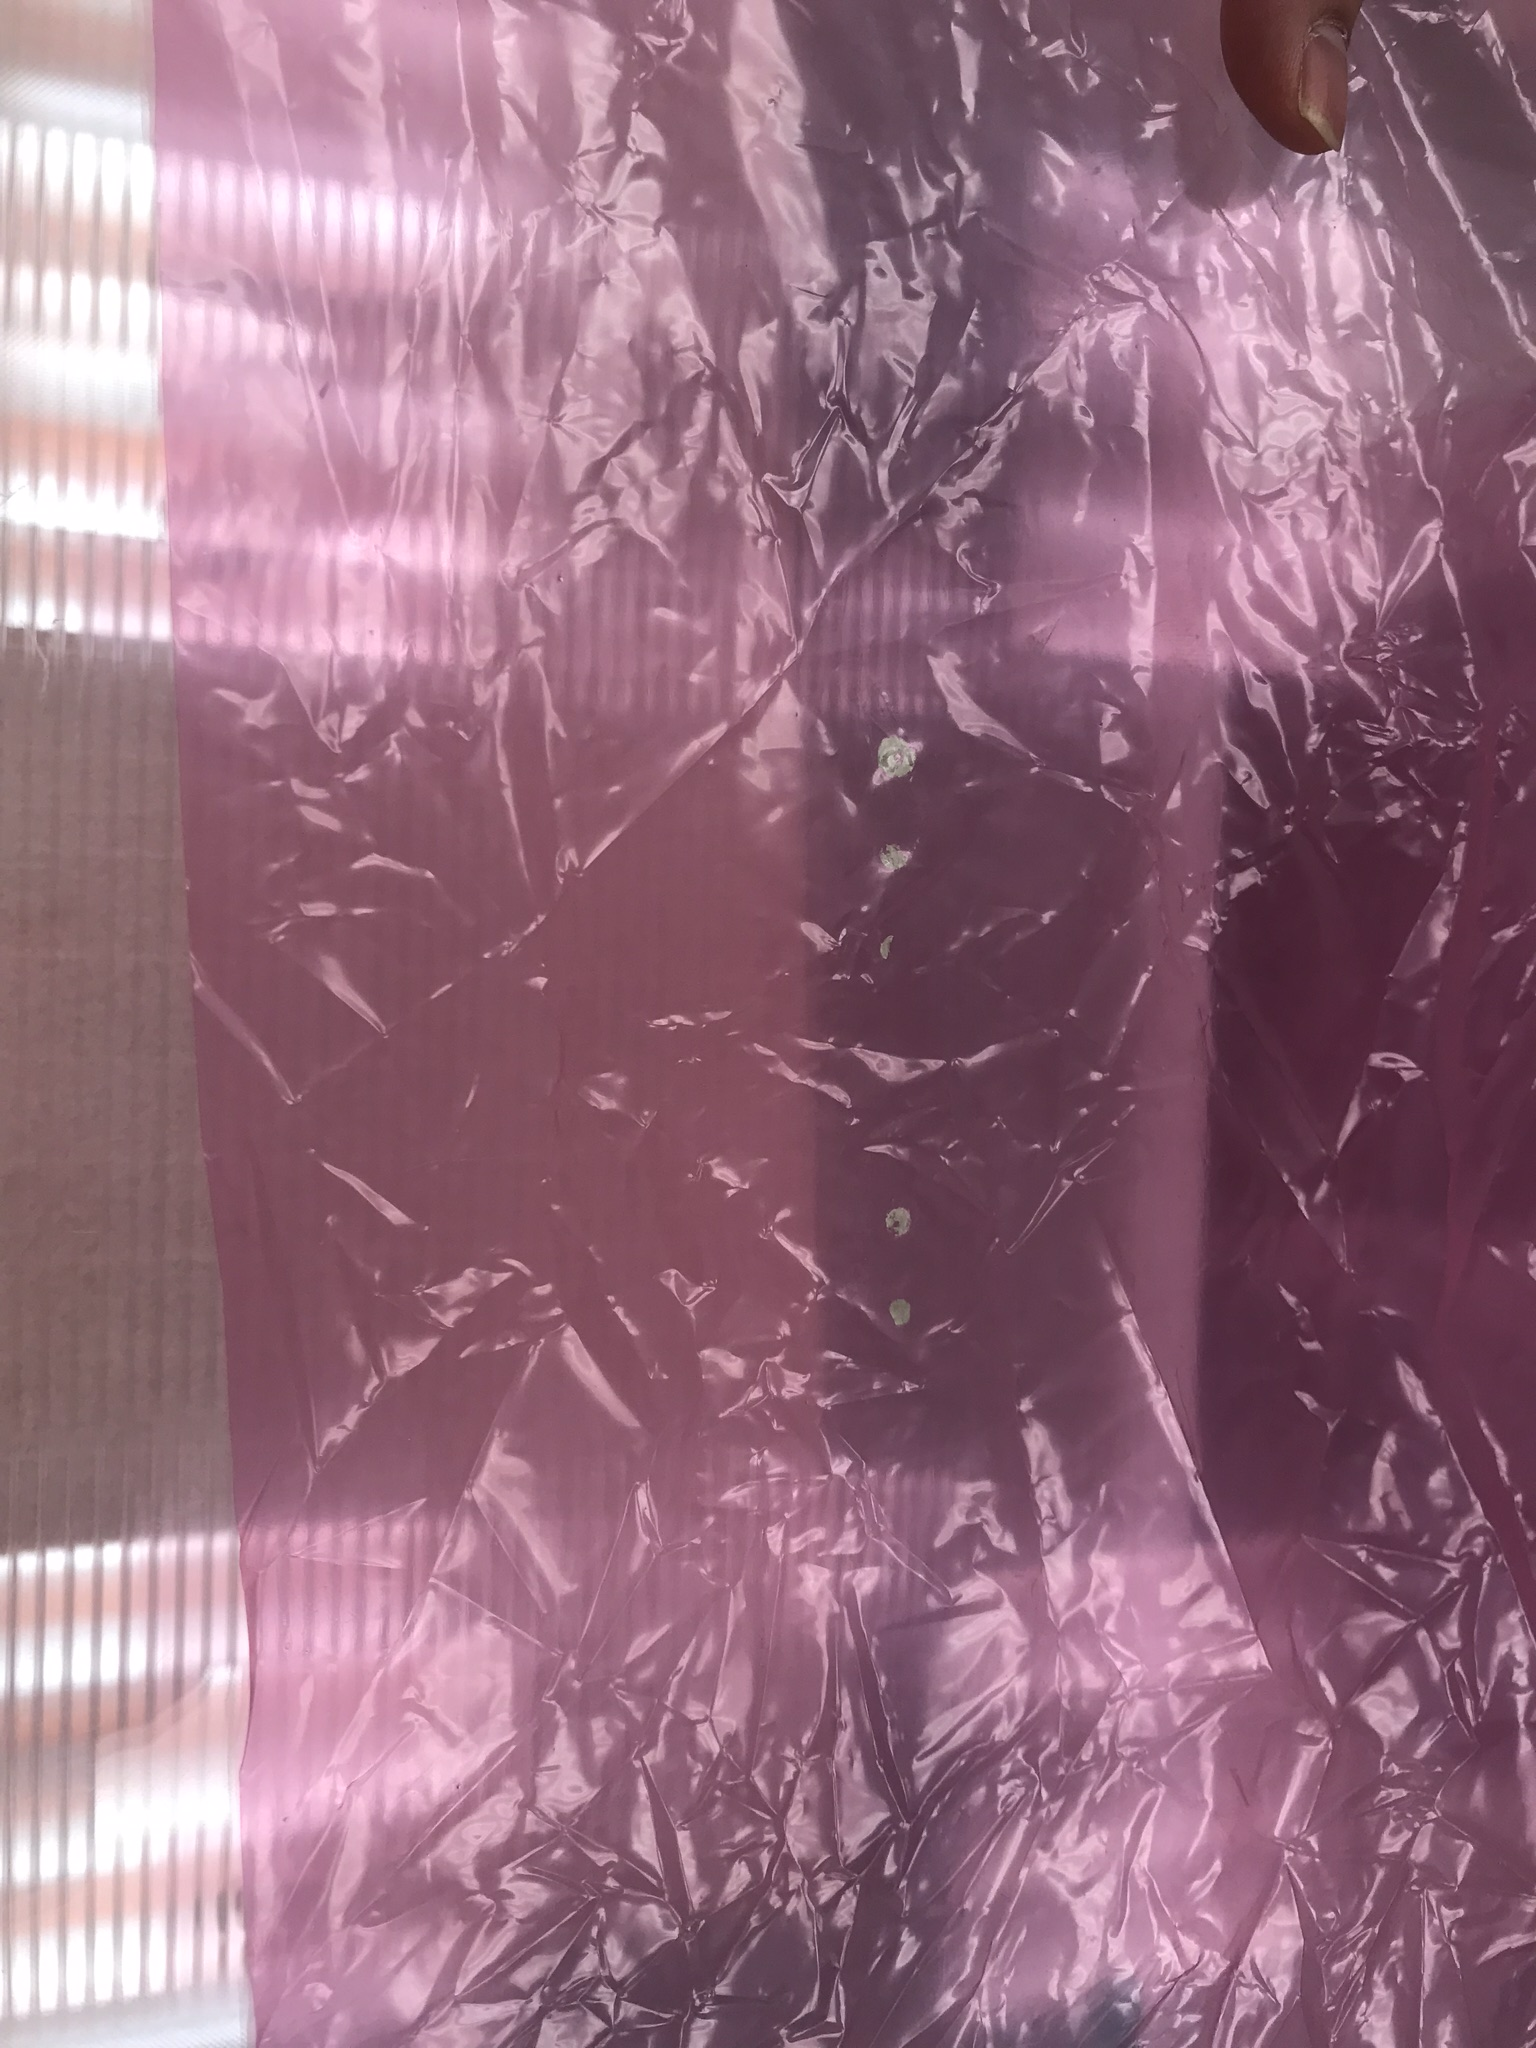
\includegraphics[width=0.40\textwidth]{Undried_Silver_Paste.jpg}
  \caption[건조되지 않은 은 페이스트]{은 페이스트가 완전히 건조되지 않은 상태에서 포장을 진행했을 때, 발생하는 현상. 방정전 필름에 은 페이스트가 묻은 것을 확인 할 수 있다. 이 때 은 페이스가 주변으로 밀려 들어가게 된다.}
  \label{fig:undried_paste}
\end{figure}
    

\begin{figure}[htb]
  \centering
  \subfloat[예제 0]{
    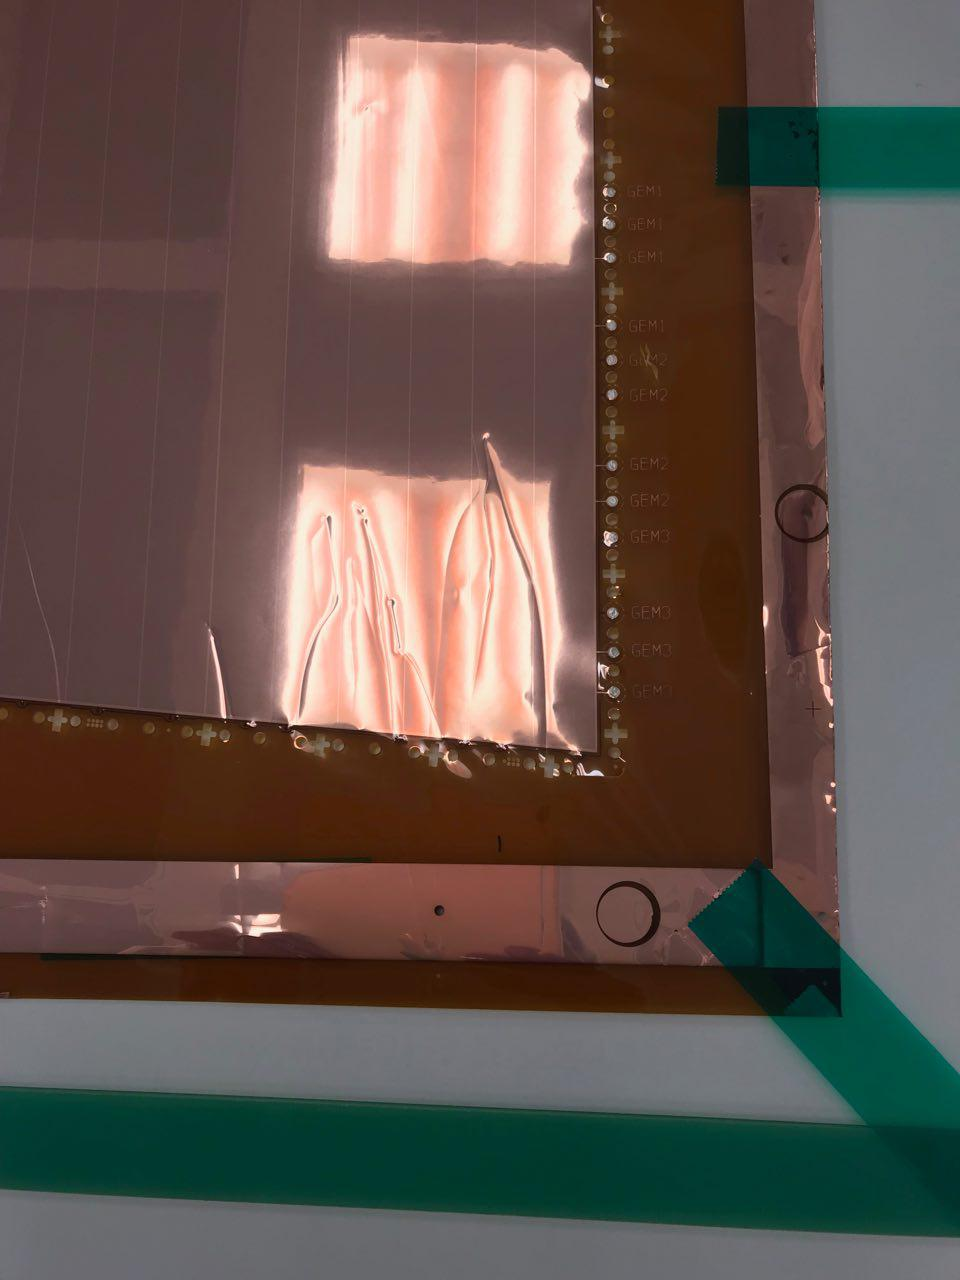
\includegraphics[width=0.40\textwidth]{damaged_case_0.jpg}
  }
  \subfloat[예제 1]{
    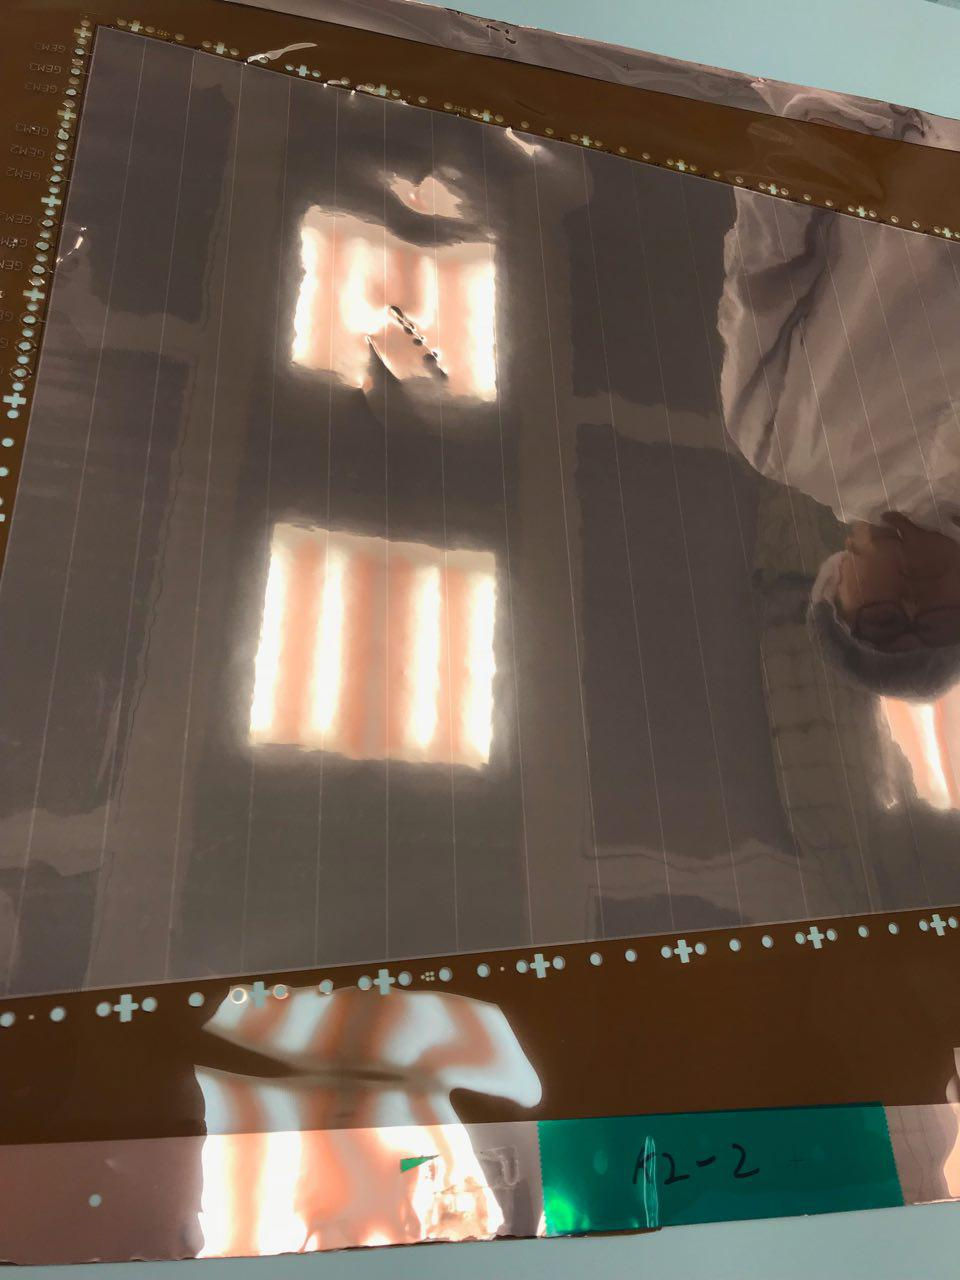
\includegraphics[width=0.40\textwidth]{damaged_case_1.jpg}
  }
  \caption[물리적 손상을 입은 포일의 예]{물리적 손상을 입은 포일의 예. 이와 같은 포일은 인수거부 할 것.}
  \label{fig:example_damaged_foils}
\end{figure}

\begin{figure}[htb]
  \centering
  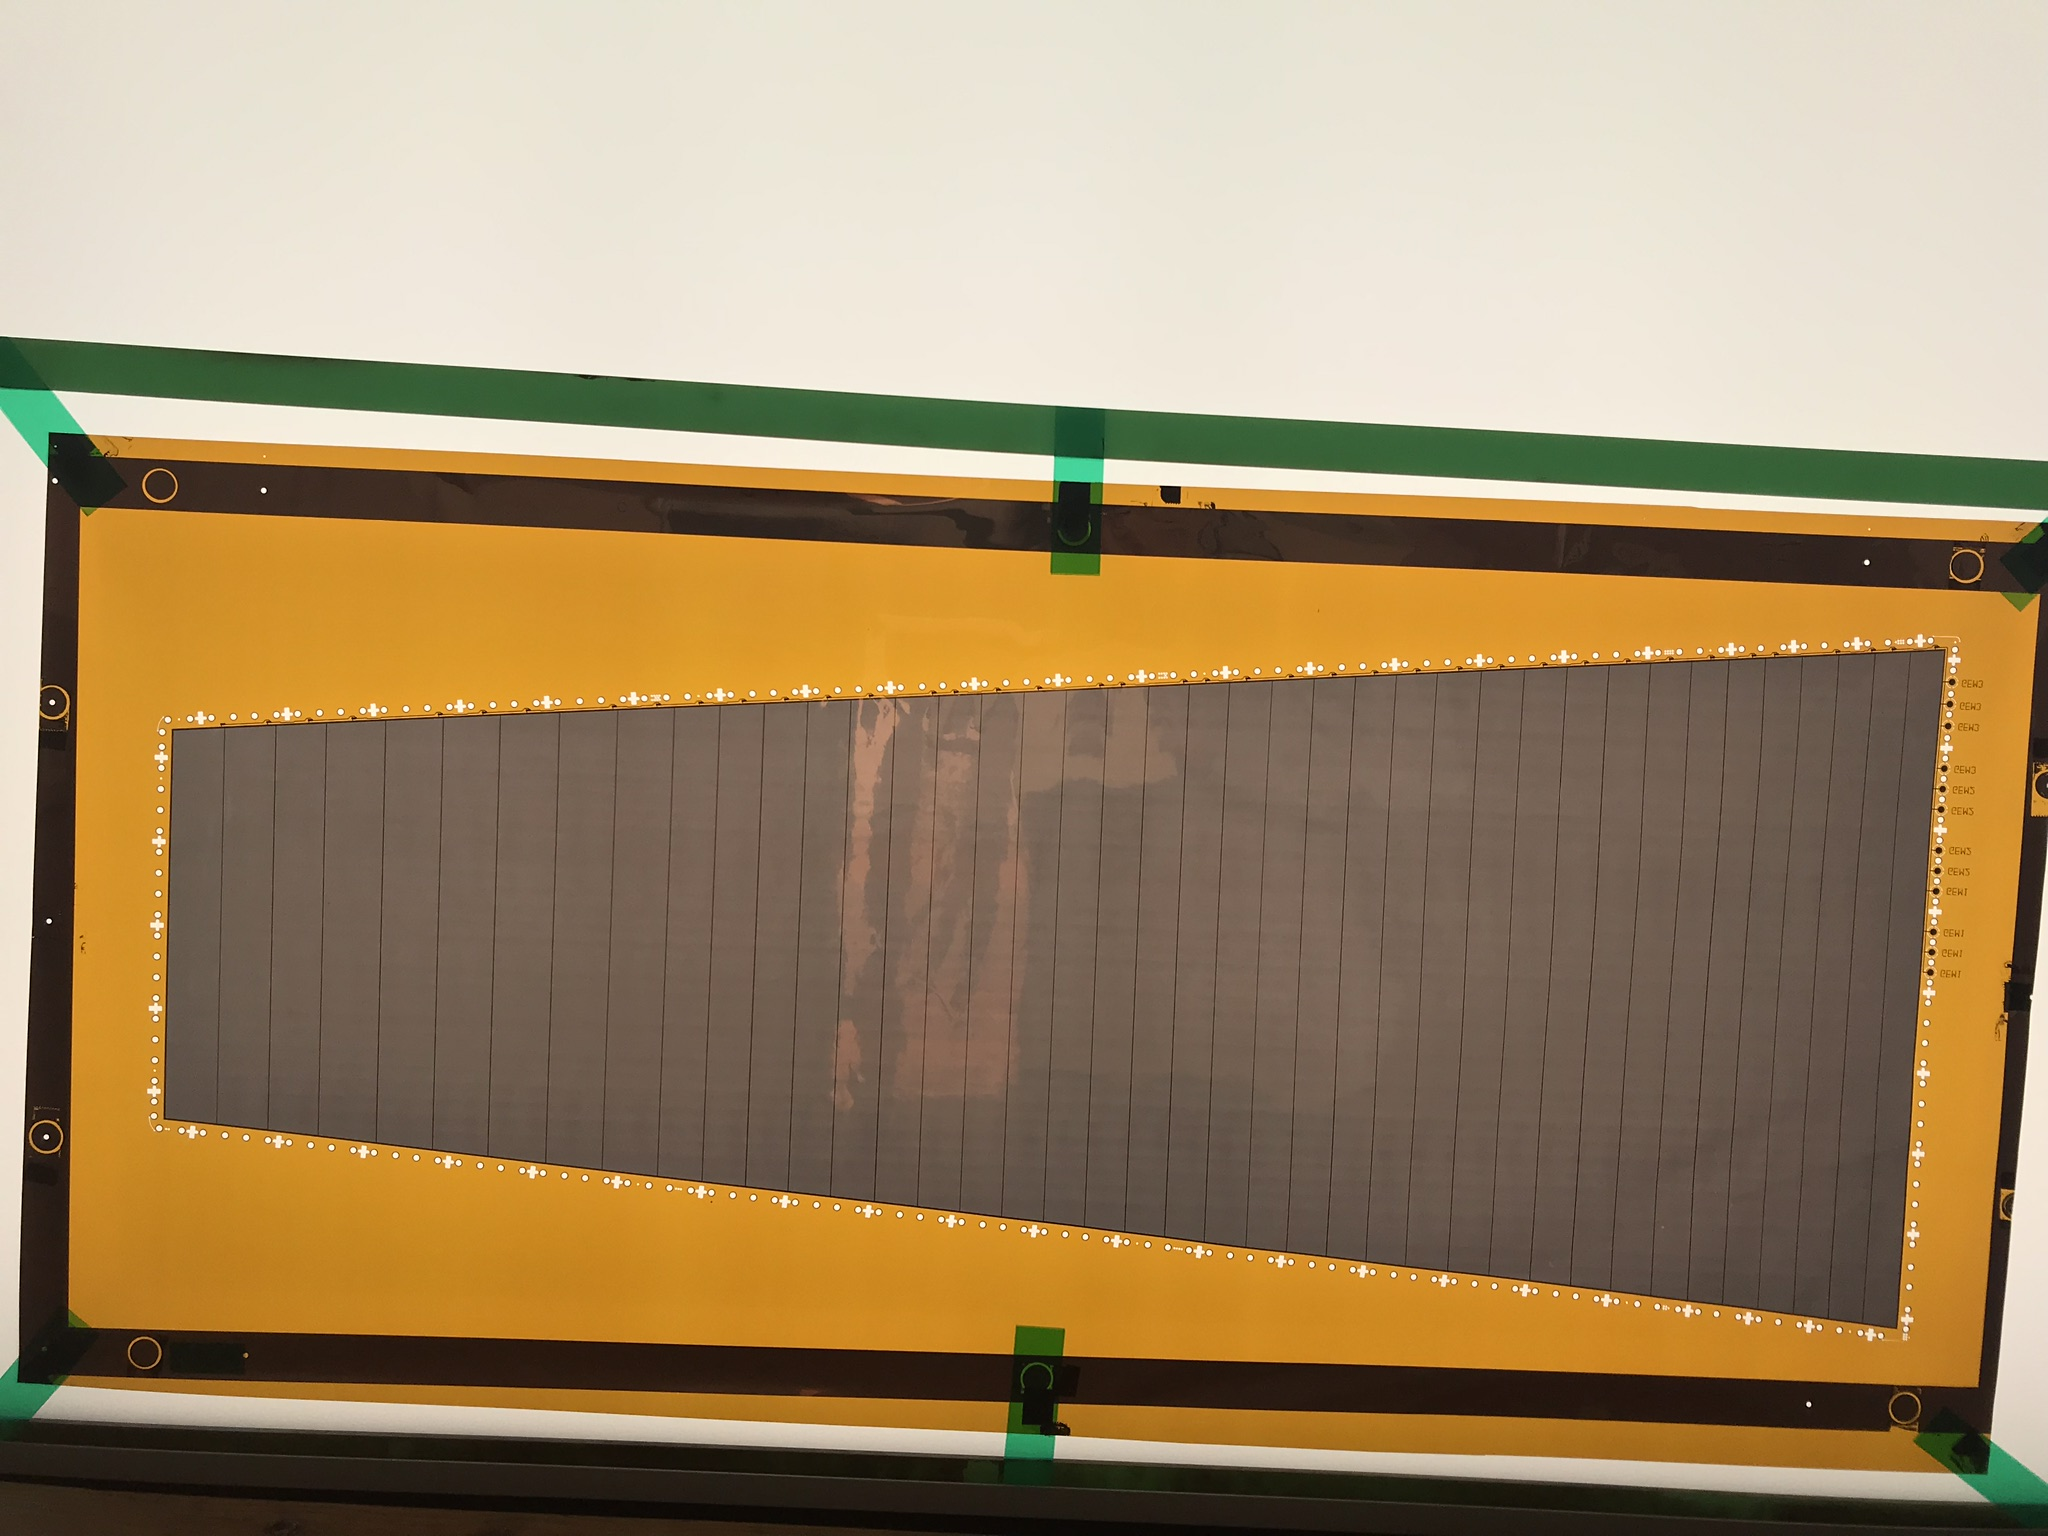
\includegraphics[width=0.60\textwidth]{Light_Board.jpg}
  \caption[대형 GEM 포일을 필름 판독기에 놓은 모습]{대형 GEM 포일을 필름 판독기에 놓은 모습. 결함이 있는 부분은 다른 곳보다 밝게 보이므로, 결함을 쉽게 확인할 수 있다.}
  \label{fig:light_board}
\end{figure}

\begin{figure}[htb]
  \centering
  \subfloat[구리층이 손상된 포일]{
    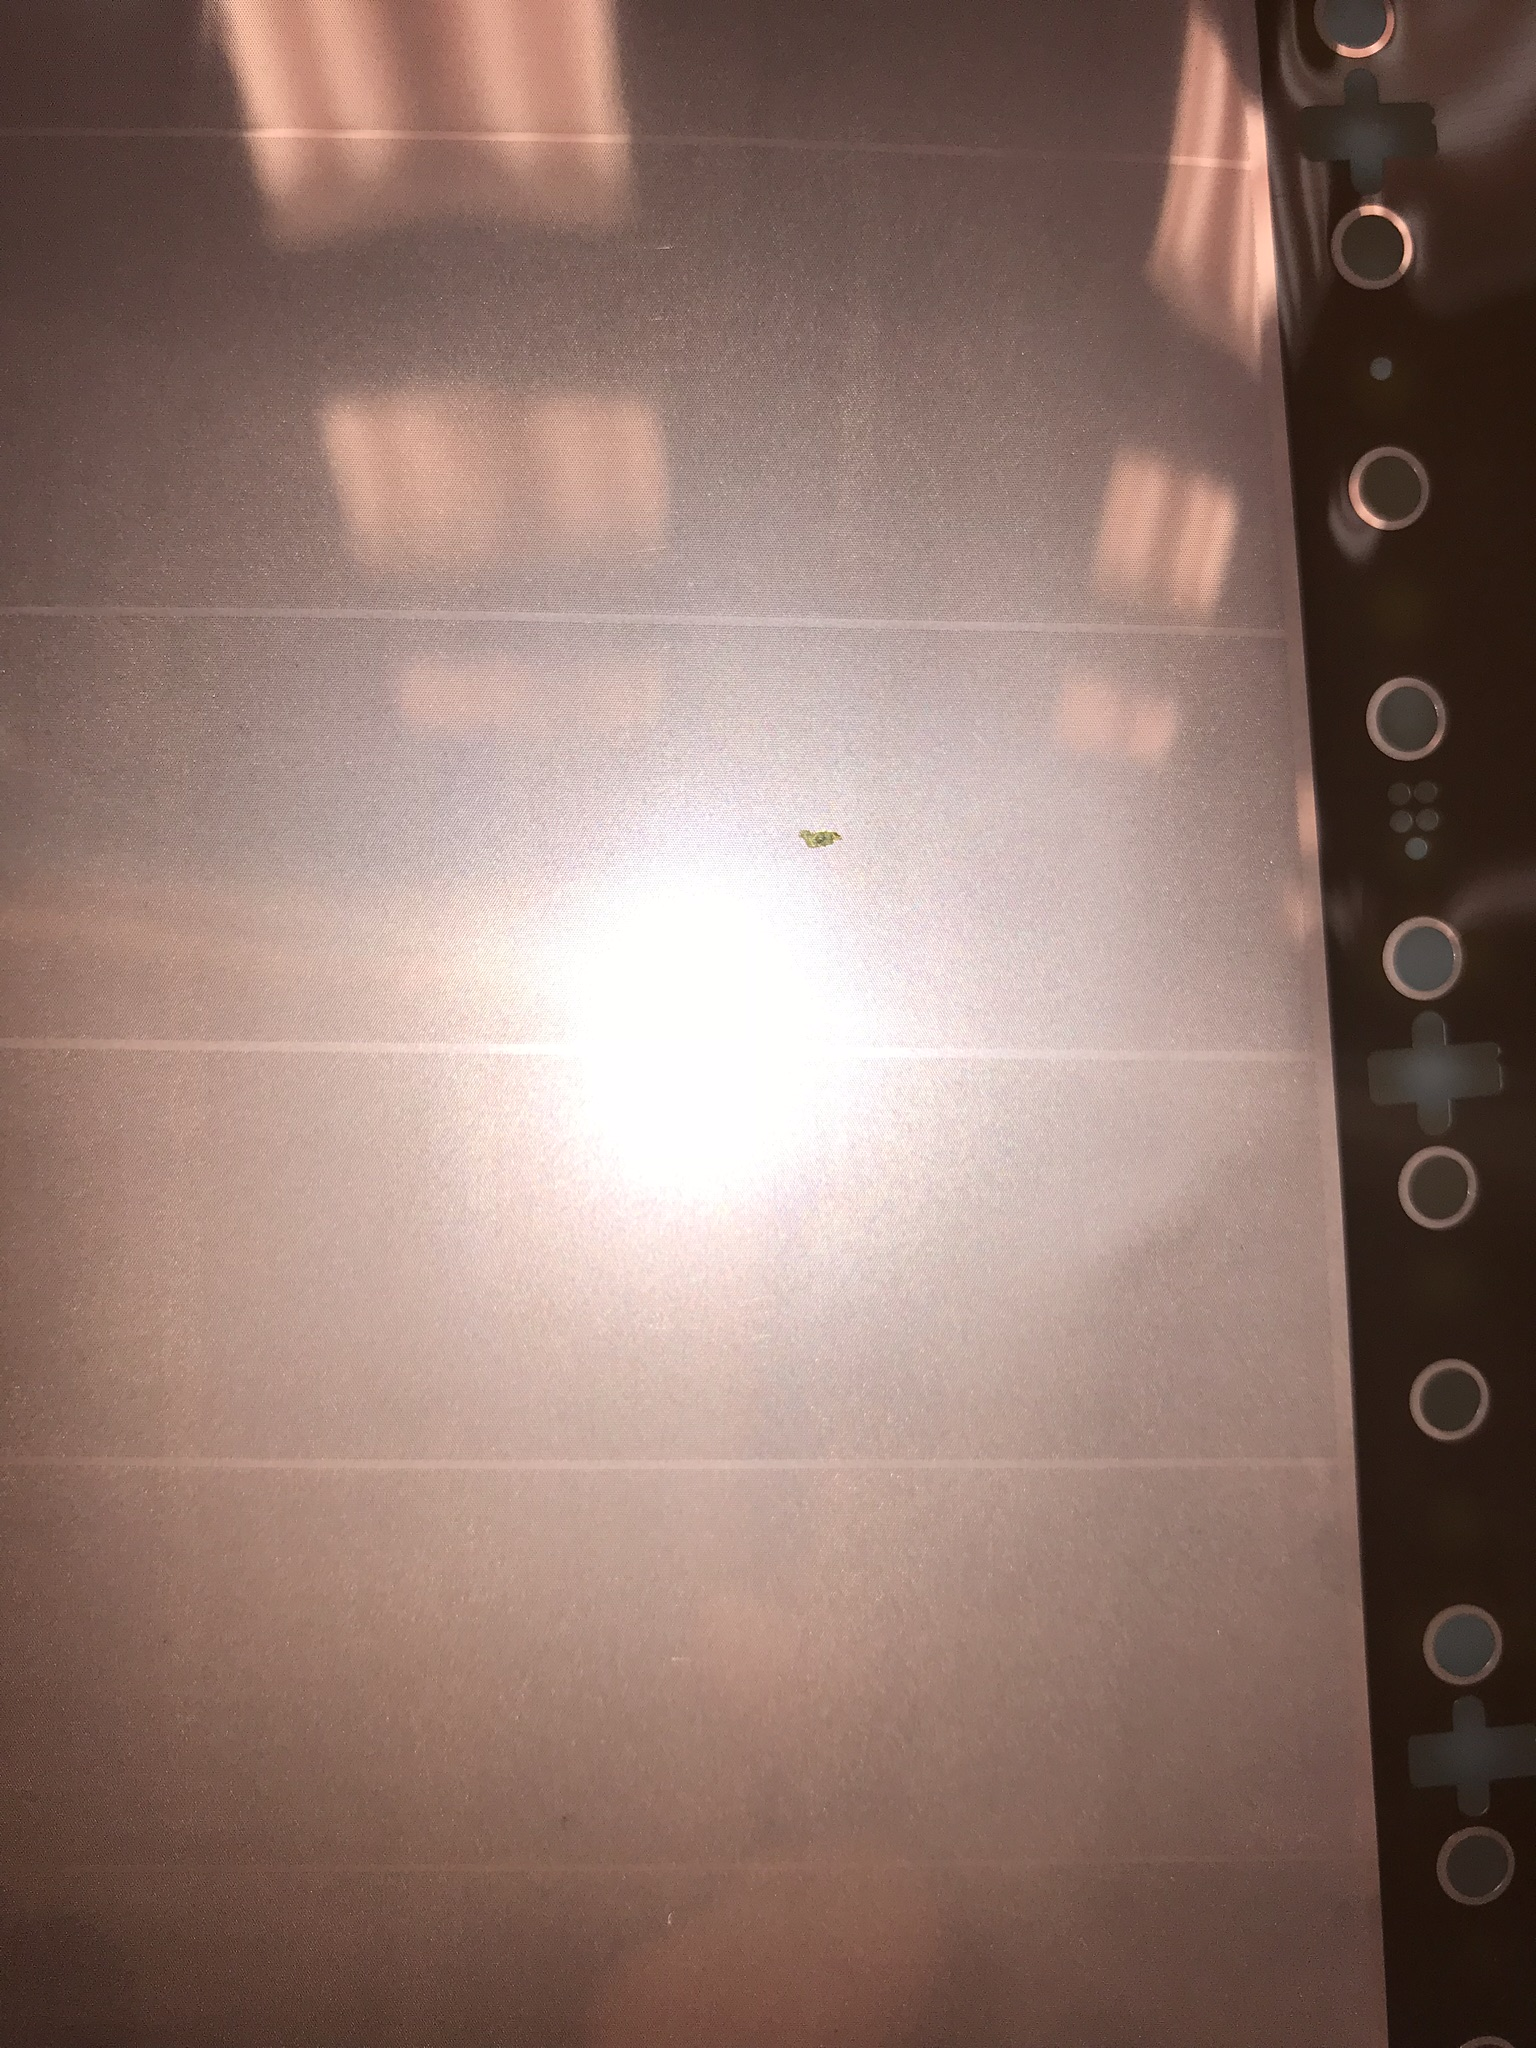
\includegraphics[width=0.40\textwidth]{Defect_OK.jpg}
  }
  \subfloat[PI층까지 손상된 포일]{
    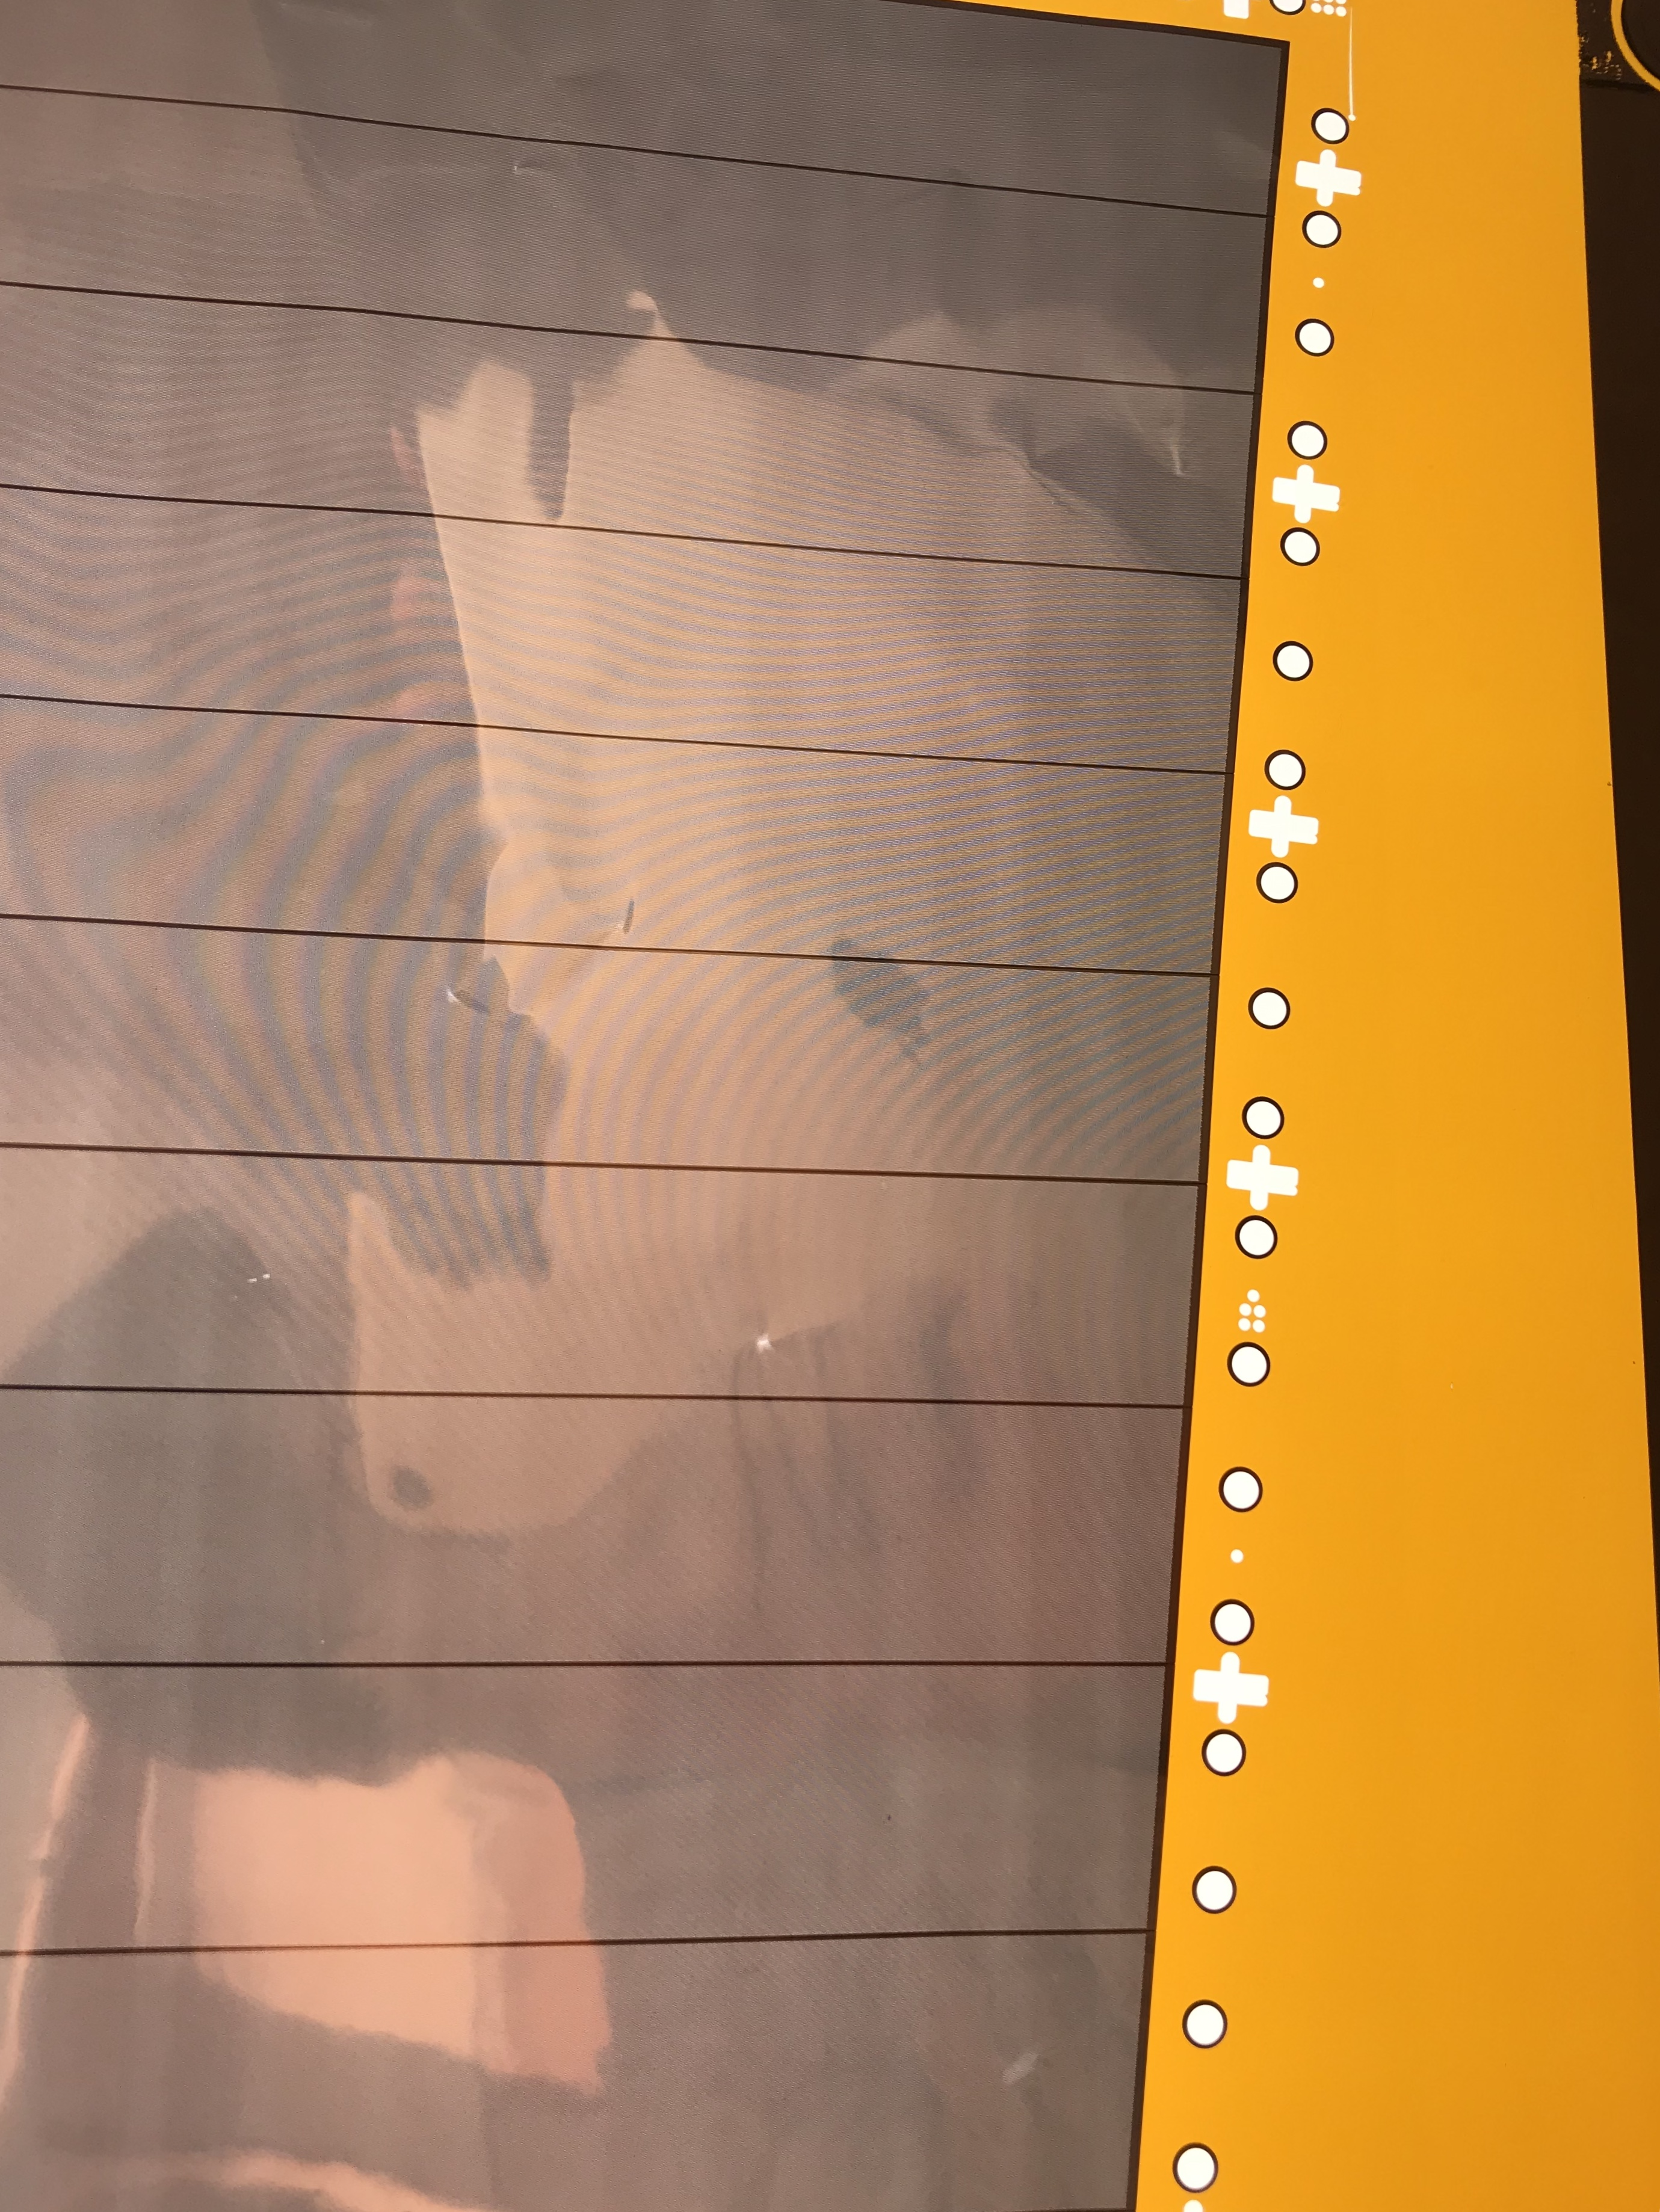
\includegraphics[width=0.40\textwidth]{Defect_Bad.jpg}
  }
  \caption[식각 결합의 예]{식각 결합의 예. 왼쪽 그림은 PI층이 온존한 경우이다. PI층이 온존하기 때문에 결함 위치가 진한 노란색으로 보인다. 이 정도 결함은 결함의 면적이 5 mm$^2$ 이하인 경우 감수 가능하다. 반면 오른쪽 그림은 PI층이 파괴되었으며 부분적으로 온전한 구리층이 사라진 PI층 위를 살짝 덮고 있는 형태이다. PI층이 사라졌기 때문에 결함 위치가 하얀색으로 보인다. 이와 같은 결함은 \uline{매우 중대한 결함으로 현미경으로 해당 부분을 면밀히 살펴보아야 한다. 그림 \protect\ref{fig:defect_bad_zoom}을 참고할 것.}}
  \label{fig:example_defect}
\end{figure}

\subsubsection{현미경을 이용한 식각 결합 양산 확인}
필름 판독기를 통한 식각 결함 검사에서 PI층이 파괴된 결함이 관찰되면 현미경을 통해 해당 위치를 면밀히 살펴야 한다. 만약 PI층의 파괴 범위보다 구리층의 파괴 범위가 더 넓어서 두 구리층이 접촉 가능성이 없는 형태라면, 결함 면적에 따라 큰 문제가 없을 수 있다. 하지만 \uline{PI층의 파괴 범위가 더 넓어서 구리층이 접촉되어 단락을 일으킬 가능성이 높은 포일은 인수거부 되어야 한다.} 그림 \ref{fig:defect_bad_zoom}은 이와 같은 치명적 결합의 양상을 보여준다.

이와 같은 치명적 결함은 구겨진 FCCL에 식각 작업을 진행했을 때 발생할 수 있는 것으로 알려져 있다. 그림 \ref{fig:defect_bad_zoom}을 보면 사진상 흐릿하지만, 포일이 구겨진 것을 확인할 수 있다. 구김으로 생긴 모서리에 결함이 위치한 것을 확인할 수 있다. 따라서 \uline{구김 위에 있는 결함이 있을 경우 매우 신중하게 검사를 진행해야 한다.}

\uline{만약 해당 치명적 결함이 발생했을 경우 메카로에 해당 결함이 발생했음을 알리고, FCCL에 구김이 발생하지 않도록  취급에 유의할 것을 부탁해야 한다. CERN에서는 해당 결함이 발생했을 경우 해당 Batch을 전부 파기할 정도로 매우 심각한 결함임을 주지시킬 것.} 

\begin{figure}[htb]
  \centering
  \subfloat[치명적 결합의 육안 사진]{
  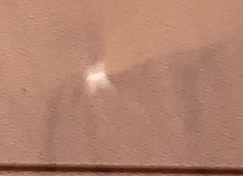
\includegraphics[width=0.40\textwidth]{Defect_Bad_Zoom.png}
  }
  \subfloat[치명적 결함의 현미경 사진]{
    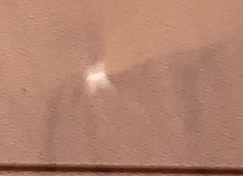
\includegraphics[width=0.40\textwidth]{Defect_Bad_Zoom.png}
  }
  \caption[치명적 식각 결함의 양상]{왼쪽 사진은 치명적 결함의 육안 사진이다. PI층이 파괴되었으며 부분적으로 온전한 구리층이 사라진 PI층 위를 살짝 덮고 있는 형태이다. PI층이 사라졌기 때문에 결함 위치가 하얀색으로 보이며, 부분적으로 온전한 구리층이 연한 갈색으로 보인다. 이런 치명적 결함은 구김으로 생긴 모서리 위에 위치한다. 오른쪽 사진은 해당 위치의 현미경 사진이다. (추후 업데이트 예정) 이와 같은 결함은 \uline{매우 중대한 결함으로 반드시 해당 포일을 인수거부해야 한다.}}
  \label{fig:defect_bad_zoom}
\end{figure}

\subsection{고전압을 이용한 검증법}
고전압을 이용한 검증법의 목표는 GEM 포일의 세척이 불량한 포일을 제거하는 것이다. 이 검증법에서 실패한 포일은 메카로에 재세척을 의뢰해야 한다.

\begin{itemize}
\item 600 V 걸기 : \uline{포일에 600 V 전압을 걸어 방전이 일어나는지 확인한다. 이 때 전원 공급 장치의 전류 한계 10 $\mu$A 이상으로 한다.} 전류 한계를 높게 설정하는 이유는 충분한 에너지를 공급하여 포일에 있는 오염이 증발하도록 하기 위함이다. 이 때 충분한 에너지가 공급되지 않으면 타다 남은 오염물이 포일에 달라 붙어서 단락을 일으킬 수 있다. \uline{600 V 전압을 걸었을 때, 5초 안에 방전이 멈추고} 수십-수백 nA의 누설전류가 관측되어야 한다. 만약 \uline{5초 후에도 지속적인 방전이 일어나거나 단락이 일어난다면, 메카로에 해당 포일의 재세척을 의뢰한다.}
\item 점진적인 공급 전압 높이기 : 600 V 걸기 검사를 통과한 포일에 대해 \uline{5 V 간격으로 공급 전압을 높여 가면서 방전이 발생하는지 확인한다.} 마찬가지로 전압을 올린 후 5초 내에 방전이 멈추어야 하며, 5초 후에도 방전이 지속될 경우 메카로에 재세척을 의뢰한다. \uline{공급 전압은 615 V까지 높인다.} 615 V의 공급 전압에도 방전이 하지 않으면 합격이다.
\end{itemize}

\subsection{QC2}
QC2은 CERN에서 정립된 포일검증법이다. 따라서 CERN과의 호환을 위해 같은 방식으로 QC2을 진행해야 한다. QC2은 10분에 걸친 QC2-Fast와 최소 7시간에 걸친 QC2-Long으로 구성된다. 포일이 \uline{QC2에서 실패하면 메카로에 해당 포일의 재세척을 의뢰해야 한다.} GEM 포일이 QC2-Long까지 통과한다면 해당 포일의 품질은 검증된 것으로 간주한다.

\subsubsection{QC2-Fast}
QC2-Fast은 빠른 시간 안에 포일의 청결도를 시험하기 위해 고안된 검증법이다. Megger MIT417/2 절연 시험기를 이용해 \uline{포일에 500 V의 공급 전압을 걸은 후, 10분에 걸쳐 포일 임피던스와 방전 횟수를 측정하는 시험이다.}

먼저 실험 환경의 \uline{상대습도와 온도를 기록}한다. 전압이 걸린 후 \uline{30초, 1분, 2분, 3분, \dots 10분이 지나는 순간의 임피던스를 기록}한다. \uline{초기 30초 이후부터 매 시간 간격 사이에 일어난 방전 횟수를 시간 간격의 뒤 시간에 기록한다.} 즉, 30초부터 1분 사이의 방전 횟수를 1분에 기록하고, 1분부터 2분 사이의 방전 횟수를 2분에 기록한다. 기록은 준비된 템플릿을 이용한다. \uline{최종적인 포일 임피던스가 10 G$\Omega$ 이상 그리고 방전 속도는 분당 1회 이하가 되어야 한다. 만약 임피던스가 낮거나 방전이 많이 일어나는 경우, 메카로에 해당 포일의 재세척을 의뢰한다.} 만약 방전 속도는 만족스러우나 최종적인 포일 임피던스가 수 G$\Omega$ 수준이라면 세척 과정 중 고압 DI수 살수 과정만 진행하여도 무방하다.     

\begin{table}[htb]
  \centering
  \begin{tabular}{|c|c|c|c|c|c|}
    \hline
    시간 (분) & 전압(V) & 저항 (G$\Omega$) & 전류 (nA) & 방전 횟수 & 총 방전 횟수\\
    \hline
    0.5 & 500 & 3.11 & 176 & - & 0\\
    1   & 500 & 3.73 & 147 & 3 & 3\\
    2   & 500 & 5.9  & 93  & 3 & 6\\
    3   & 500 & 7.6  & 72  & 1 & 7\\
    4   & 500 & 8    & 68  & 2 & 9\\
    5   & 500 & 8.5  & 64  & 1 & 10\\
    6   & 500 & 9.2  & 59  & 0 & 10\\
    7   & 500 & 9.6  & 57  & 0 & 10\\
    8   & 500 & 10.5 & 52  & 0 & 10\\
    9   & 500 & 10   & 55  & 0 & 10\\
    10  & 500 & 11   & 50  & 0 & 10\\
    \hline
  \end{tabular}
  \caption[일반적인 QC2-Fast 검증 결과]{일반적인 QC2-Fast 검증 결과. 축전이 진행되면서 저항이 시간에 따라 올라가는 것이 정상적인 현상이다. 방전이 일어나면서 포일에 앉은 오염물이 타고 이로 인해 저항이 갑자기 올라가는 경우도 흔하다.}
  \label{tab:example_qc2_fast_result}
\end{table}
  
\subsubsection{QC2-Long}
QC2-Long은 포일의 장기간 안정성을 시험하기 위해 고안된 검증법이다. \uline{GEM 포일이 QC2-Long까지 통과한다면 해당 포일의 품질은 검증된 것으로 간주한다.} QC2-Long은 건조 환경에서 진행해야 한다. 따라서 QC2-Long은 이를 위해 고안된 건조 질소 박스에서 진행된다. 포일을 건조 질소 박스에 넣은 후 SHV 케이블을 연결한다. 질소 박스를 닫고, 질소를 흘린다. QC2-Long을 진행할 수 있는, 상대습도 7\%에 떨어질 때까지 수 시간에서 수십 시간이 걸린다. 따라서 해당 검증은 시간  계획을 잘 세워서 진행해야 한다. 장기간의 걸친 검사를 진행하기 위해 QC2-Long은 컴퓨터로 제어되어 진행된다. 제어와 기록을 위한 SW은 \url{https://github.com/diracyoon/GEM_QC_SW}에서 다운 받을 수 있다. 해당SW의 컴파일과 실행법은 \url{https://github.com/diracyoon/GEM_QC_SW}의 README 파일을 참조할 것.

상대습도가 떨어지기를 기다리며 Preparation\_QC2\_Long을 실행한다. Preparation\_QC2\_Long은 장시간에 걸쳐 점진적으로 450 V에서 615 V까지 전압을 높인다. 각 전압 단계에서 전압이 방전 없이 10분간 유지되면, 전압을 높여 다음 단계로 넘어간다. 만약 한 단계에서 3회 초과의 방전이 일어나면, 해당 전압에서 검사가 실패되고 전압을 낮추어 이전 단계로 돌아간다. 만약 한 전압에서 3회 초과의 실패가 일어나면 Preparation\_QC2\_Long은 실패한 것으로 간주되고 비정상 종료된다. 비정상적으로 Preparation\_QC2\_Long가 종료되면 HV 모듈의 전원이 꺼진다. 반면 포일이 Preparation\_QC2\_Long을 성공적으로 통과하여 Preparation\_QC2\_Long이 정상적으로 종료된 경우, 615 V의 전압이 유지된다. 만약 \uline{잦은 방전으로 Preparation\_QC2\_Long이 비정상 종료된 경우 메카로에 해당 포일의 재세척을 의뢰한다.}

GEM 포일이 Preparation\_QC2\_Long을 통과했고, 질소 박스내 상대 습도가 7\% 이하로 떨어지면, QC2\_Long을 시도할 수 있다. QC2\_Long이 실행되면 600 V와 100 V을 반복하는 스트레스 테스트를 5회 실시 후, 6시간에 걸쳐 600 V의 전압을 포일에 걸어 주고 누설 전류와 방전 속도를 측정한다. 마지막 단계가 QC2\_Long의 핵심적인 단계이다. 이때 \uline{누설전류가 3 nA 이하로 안정적으로 유지되어야 하며, 방전은 3회 이하로 일어나야 한다. 만약 지나치게 크거나 안정적이지 않은 누설 전류가 관찰되거나, 3회 초과의 방전이 관찰되면 메카로에 해당 포일의 재세척을 의뢰한다. 3회 초과의 방전이 일어날 경우, QC2\_Long은 비정상 종료된다.} 만약 방전 없이, 수 nA의 목표치를 약간 상회하는 안정적인 누설 전류가 관측되었을 경우, 세척 과정 중 고압 DI수 살수 과정만 진행하여도 무방하다.

Monitor SW을 통해 진행 중인 그리고 완료된 Preparation\_QC2\_Long와 QC2\_Long의 결과를 확인할 수 있다. Monitor는 현재 진행 중인 품질 검증 프로세스의 유무를 감시한다. 만약 진행 중인 프로세스가 있다면, TCanvas GUI에 각 HV 채널 별로 subpad에 그 결과를 표시한다. 프로세스가 완료되면, 정상 또는 비정상 종료에 관계 없이, 그 결과가 Monitor에 의해 Output 폴더에 저장된다.   

  
\section{포장법}
세척이 끝난 포일이 배송 중 다시 오염 되거나 파손되는 것을 막기 위해 올바른 포장법을 적용하는 것이 중요하다. \uline{포일 포장에서 가장 신경 써야할 것은 먼지를 제거하는 것과, 포일이 구겨지지 않게 고정하는 것이다.} 포일 포장법은 제공되는 동영상을 참고할 것. 본 문서에서는 주요 사항에 대해서만 간략하게 기술한다.

포장의 외곽은 폴리카보네트 판을 이용해 물리적 지지대의 역할을 하게 한다. 압력과 SMD 저항에 의해 포일이 인접한 포일을 상하게 하는 것을 막기 위해 포일 사이에는 폼을 깔아 준다. \uline{폼의 크기는 포일이 구겨지는 것을 막기 위해 반드시 포일보다 커야한다.} 포일은 방전 필름으로 감싸 준다. 포장에 사용되는 모든 요소는 청소기와 DCR 롤러를 이용해 청소한다. 배송 중 포일이 움직이는 것과 구김이 발생하는 것을 막기 위해, 폴리카보네이트 판에 모든 요소의 네 뒤퉁이를 3M PET 테이프로 고정한다. \uline{완성된 포장팩은 청소된 비닐 봉투에 담아 외부 먼지가 유입되는 것을 막는다.} 최대 12장의 포일을 한 팩에 담을 수 있다.     

\begin{figure}[htb]
  \centering
  \subfloat{
    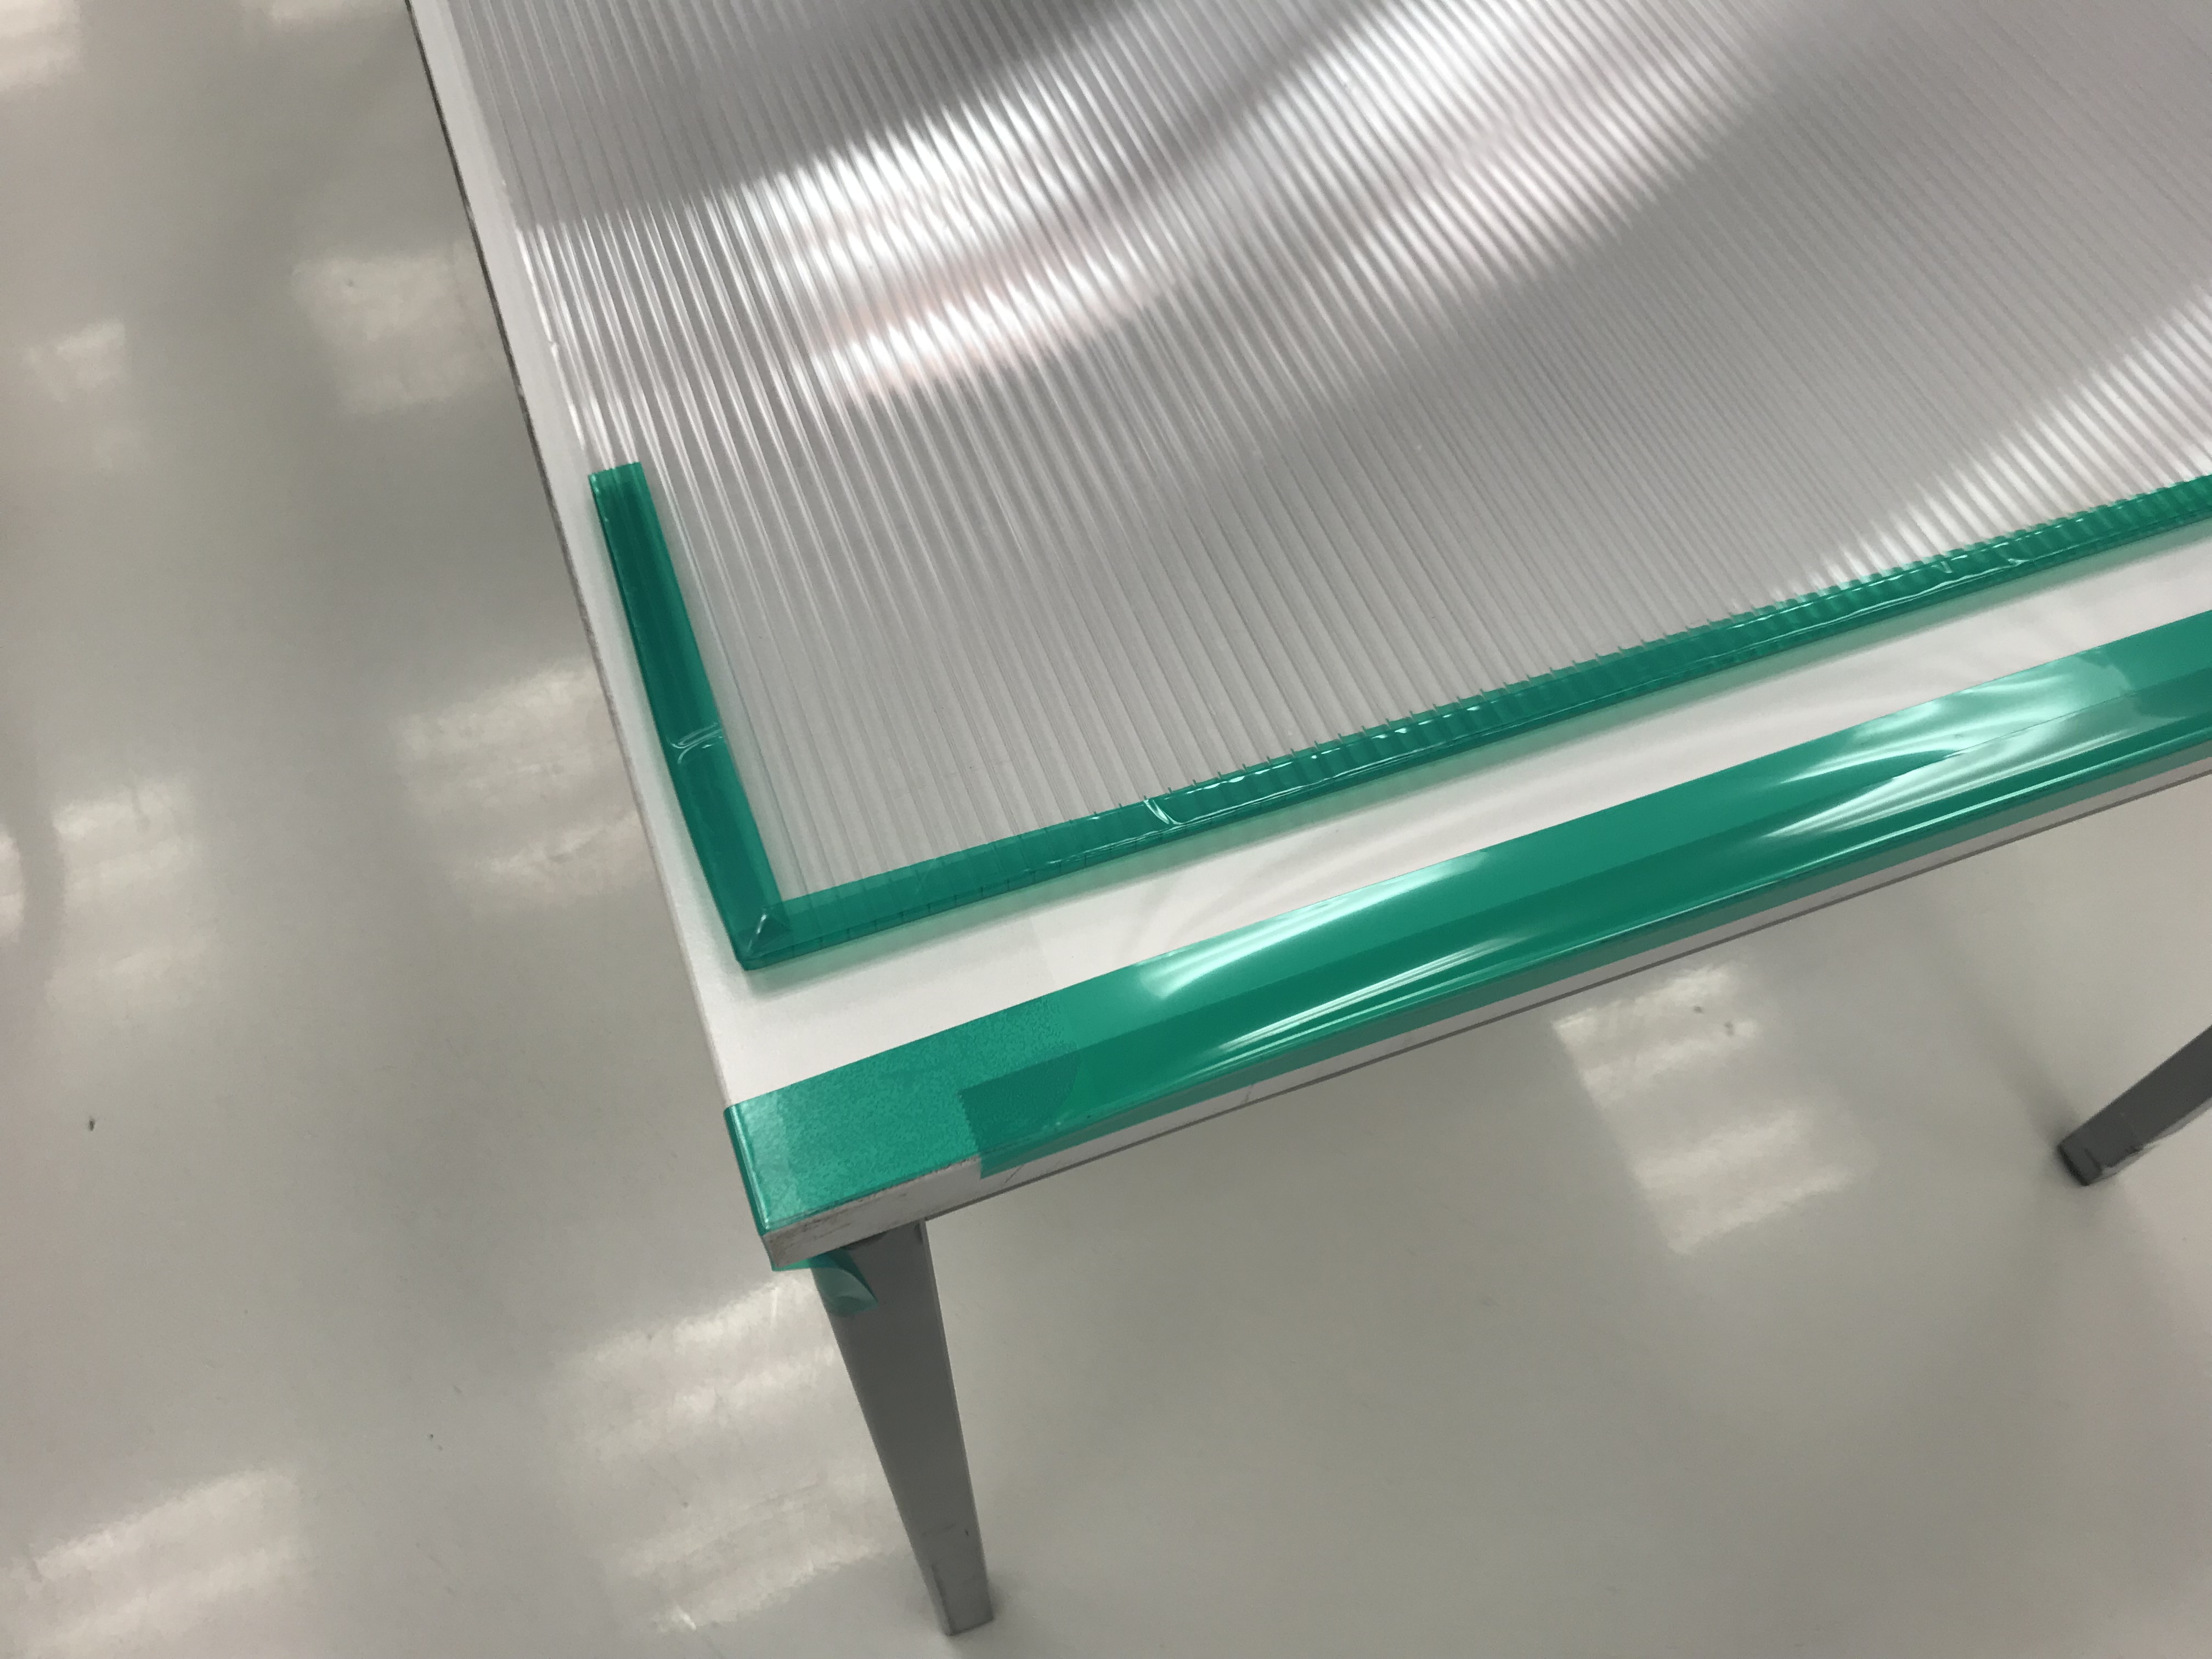
\includegraphics[width=0.40\textwidth]{PolyCarbonate.jpg}
  }
  \subfloat{
    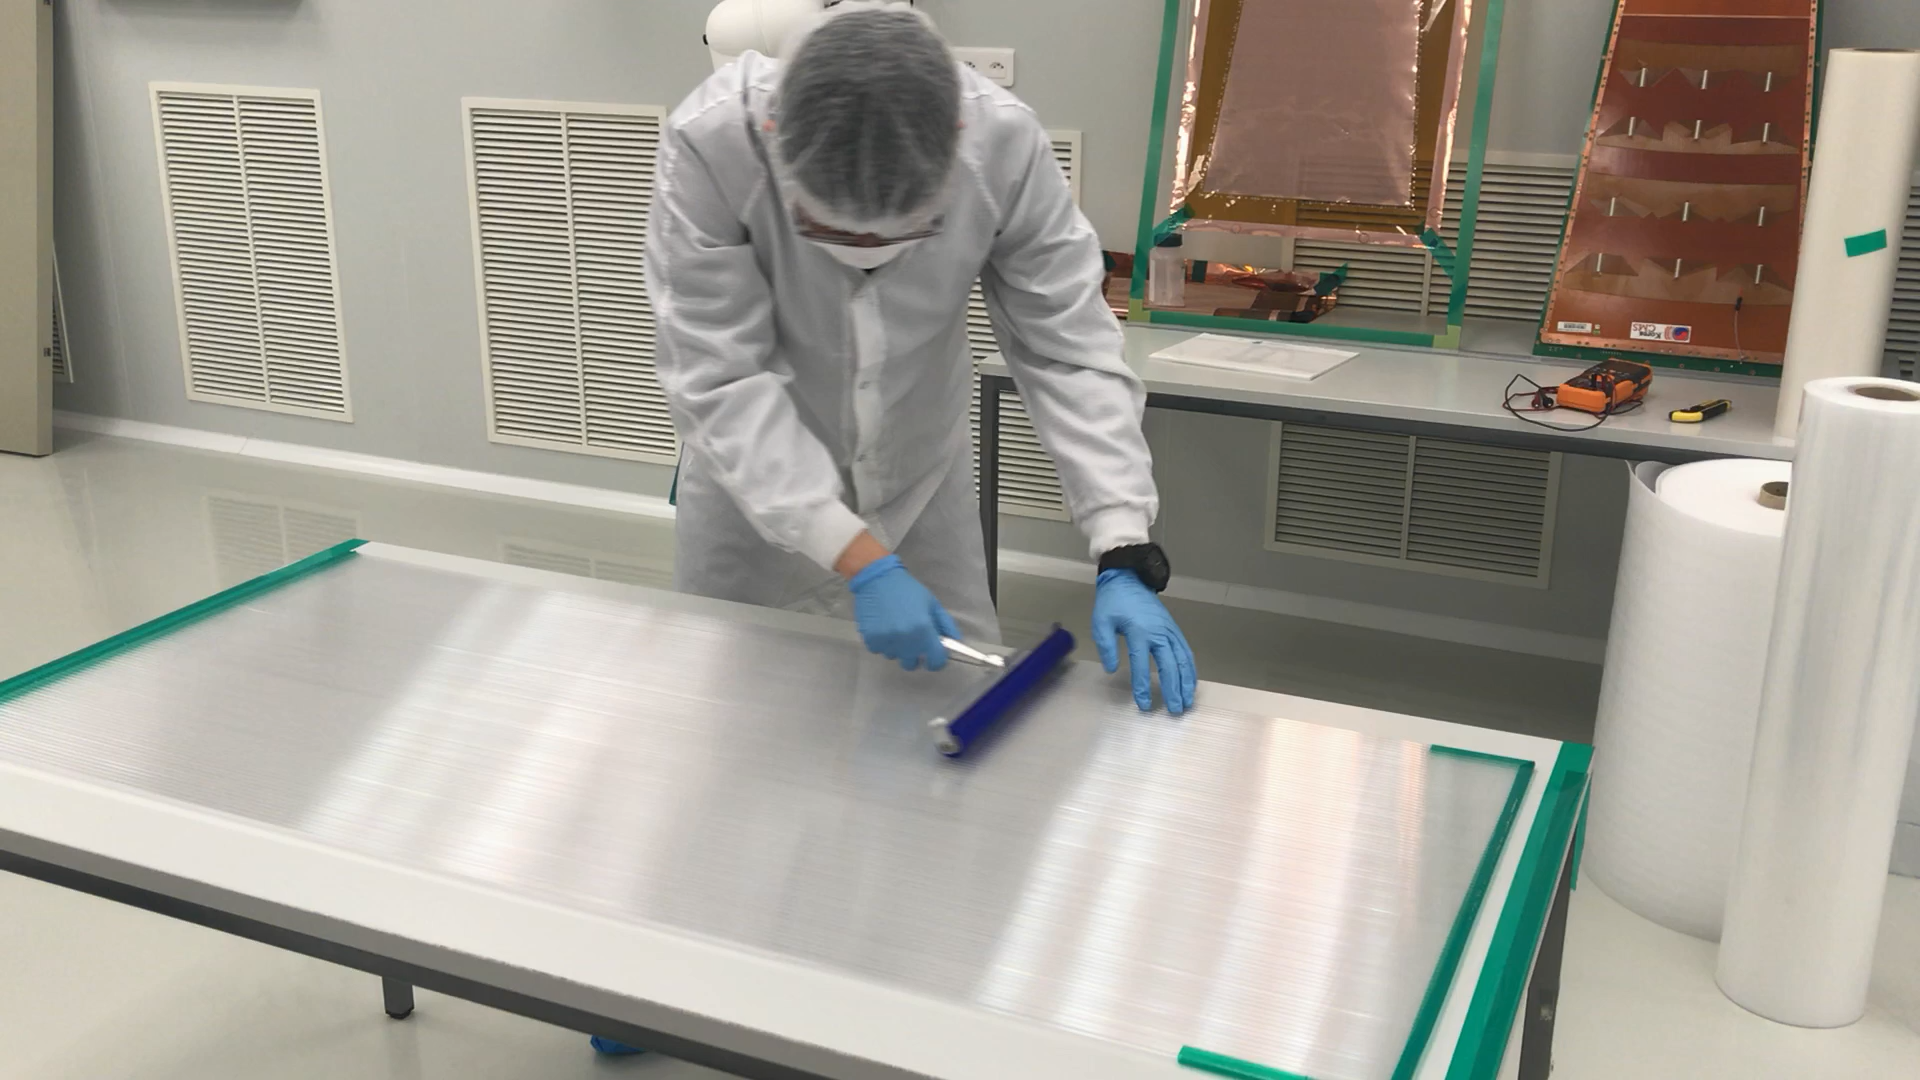
\includegraphics[width=0.40\textwidth]{Cleaning_Polycarbonate.png}
  }
  \caption[폴리카보네이트 판의 절단면 처리]{왼쪽 : 폴리카보네이트 판의 절단면은 부스러기가 나오는 것을 막기 위해 3M PET 테이프로 막아준다. 오른쪽 : 폴리카보네이트 판은 DCR 롤러로 양면을 청소한다.}
  \label{fig:polycarbonate}
  \end{figure}

\begin{figure}[htb]
  \centering
  \subfloat{
    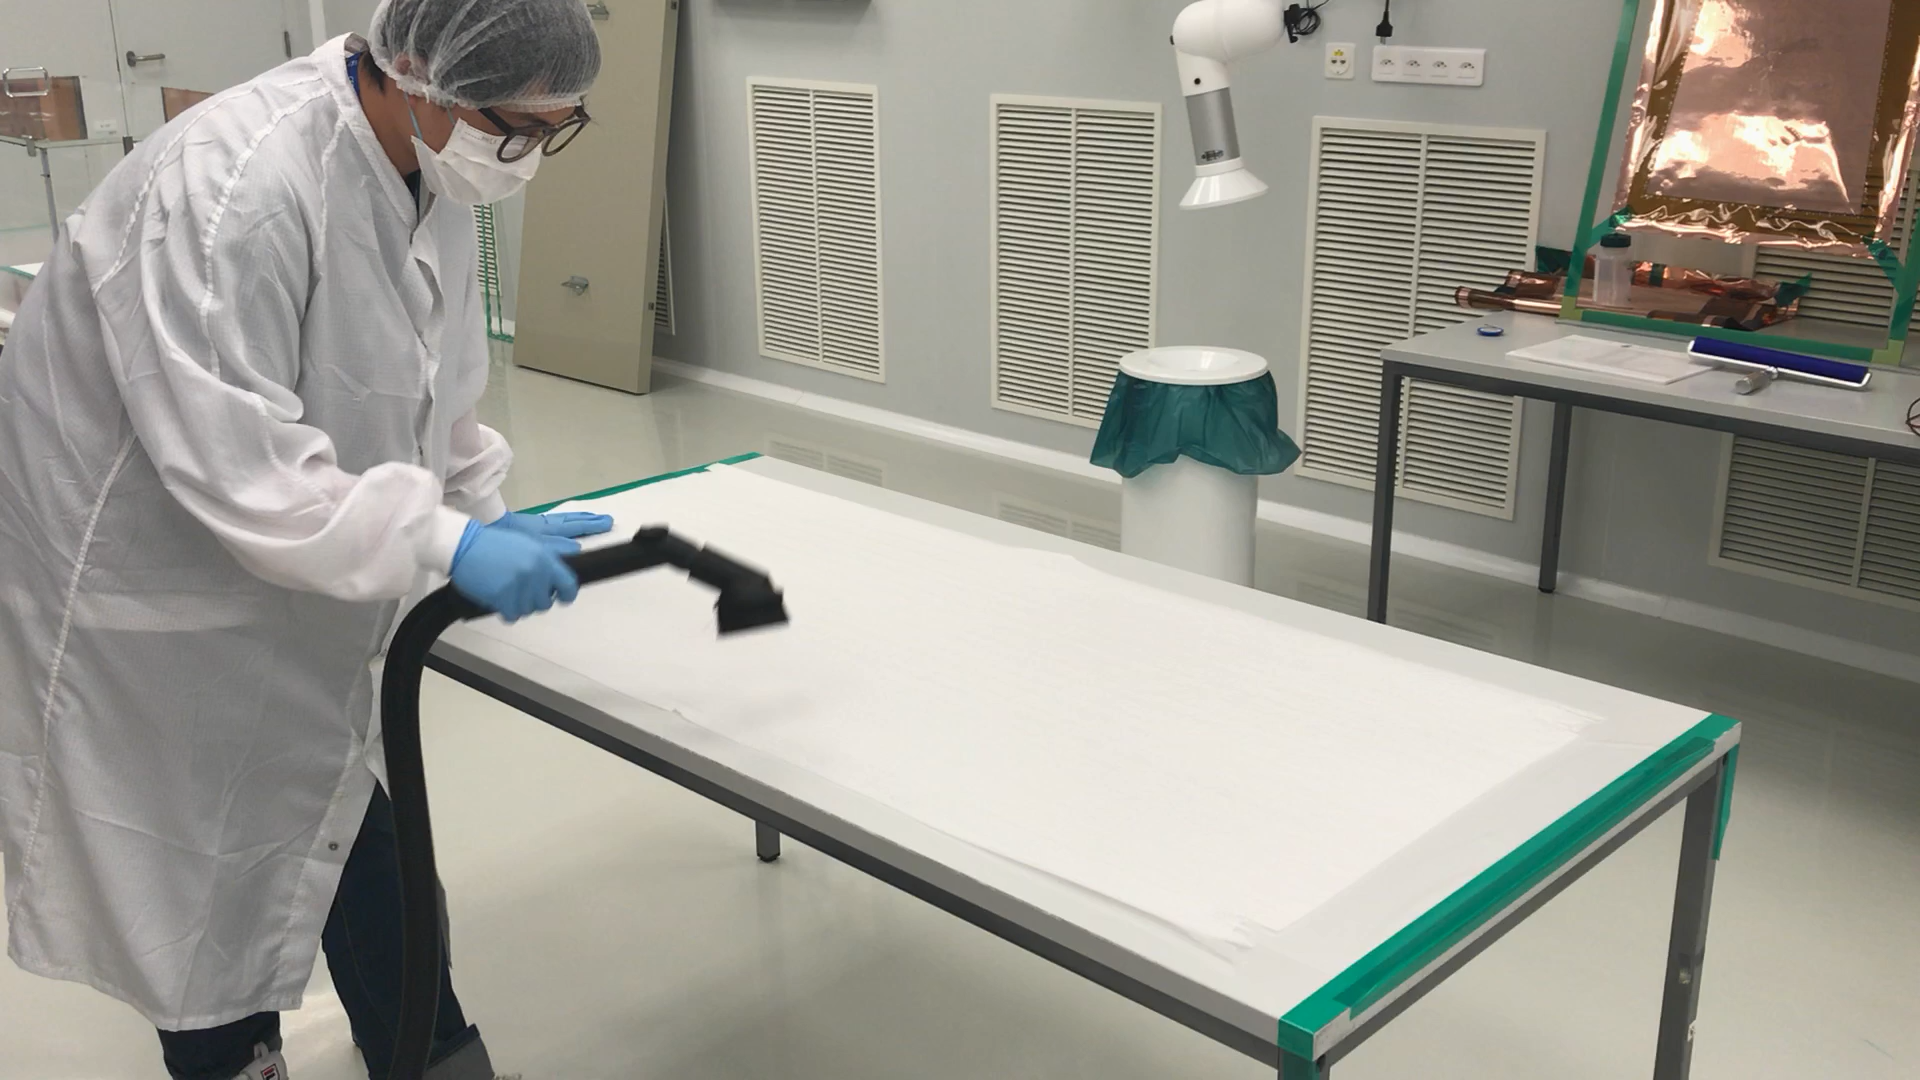
\includegraphics[width=0.40\textwidth]{cleaning_foam.png}
  }
  \subfloat{
    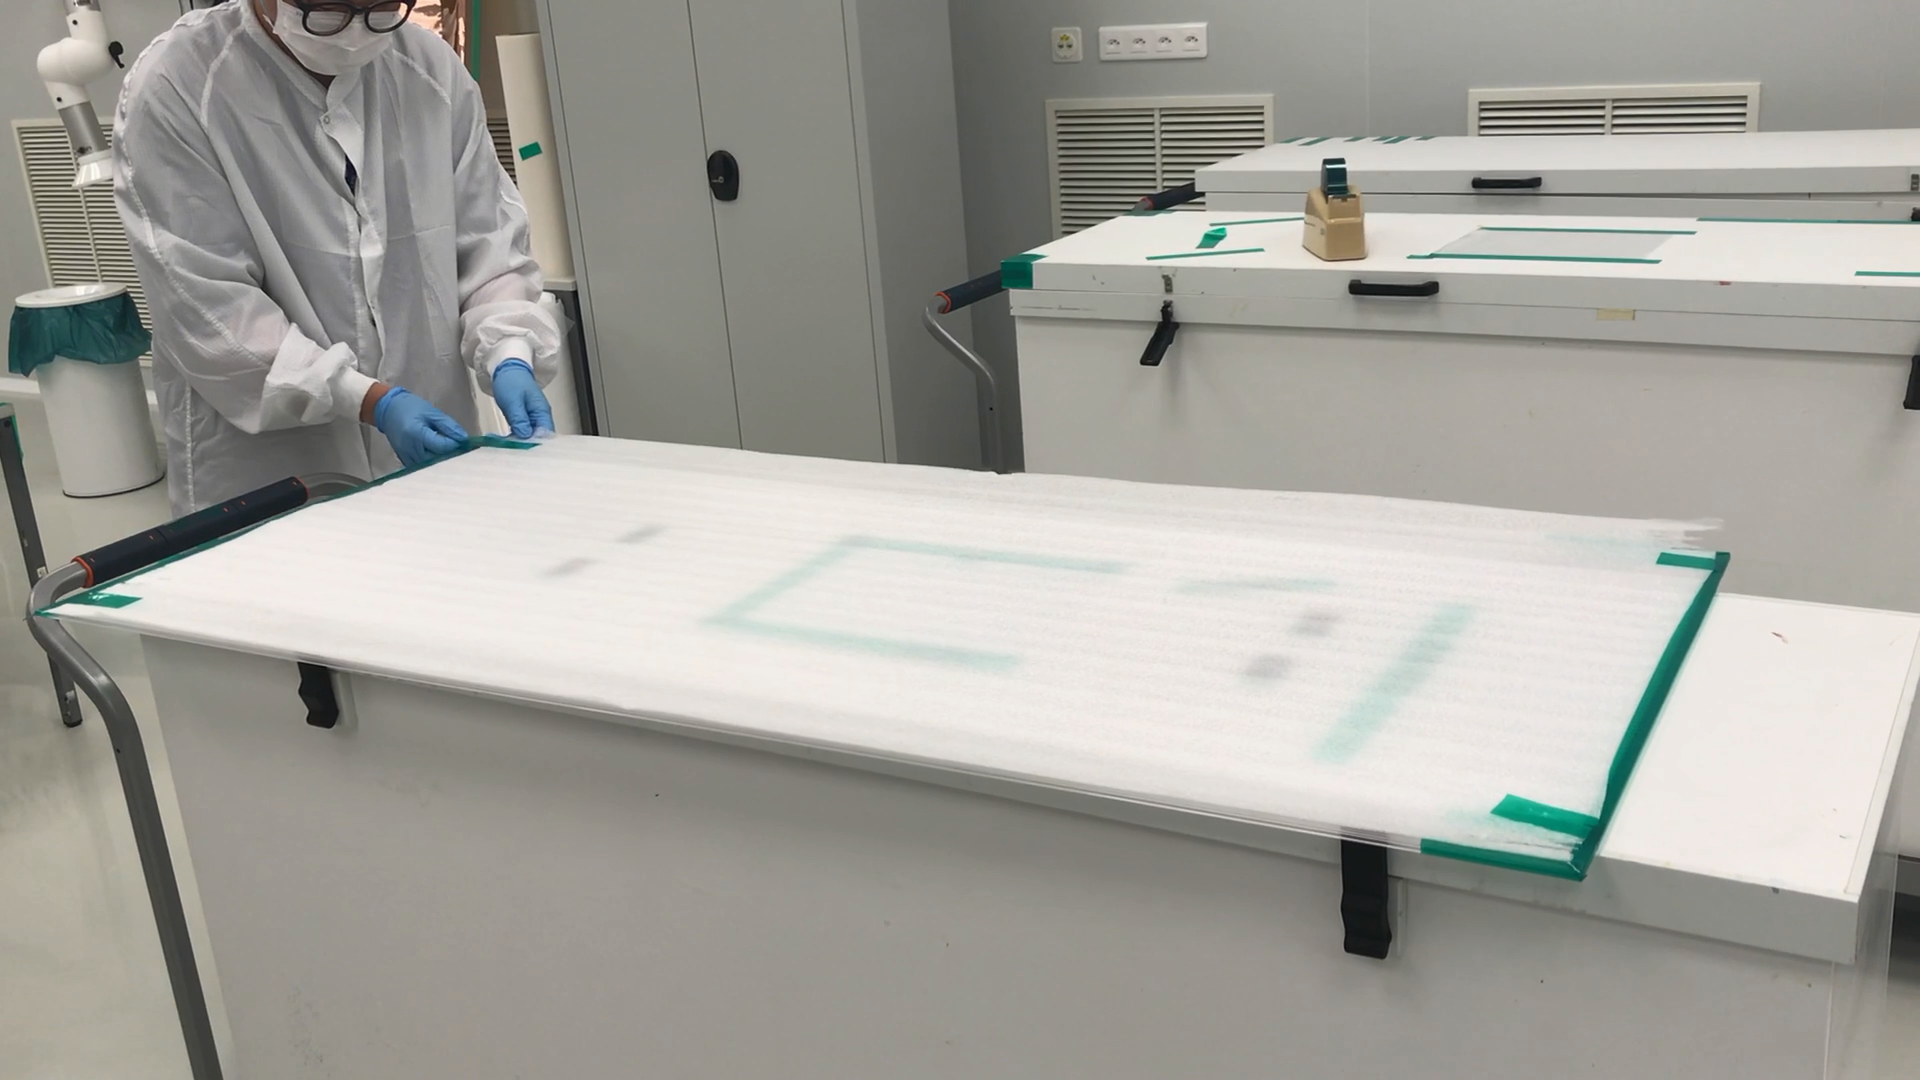
\includegraphics[width=0.40\textwidth]{fixing_foam.png}
  }
  \caption[폼의 처리]{왼쪽 : 폼은 청소기를 이용해 청소한다. \uline{폼의 크기는 포일이 구겨지는 것을 막기 위해, 최소 반드시 포일의 크기보다는 커야한다.} 오른쪽 : 폼은 폴리카보네이트 판에 3M PET 테이프로 네 뒤퉁이를 고정한다. 이 때, 구김이 없어야 한다.}
  \label{fig:foam}
\end{figure}

\begin{figure}[htb]
  \centering
  \subfloat{
    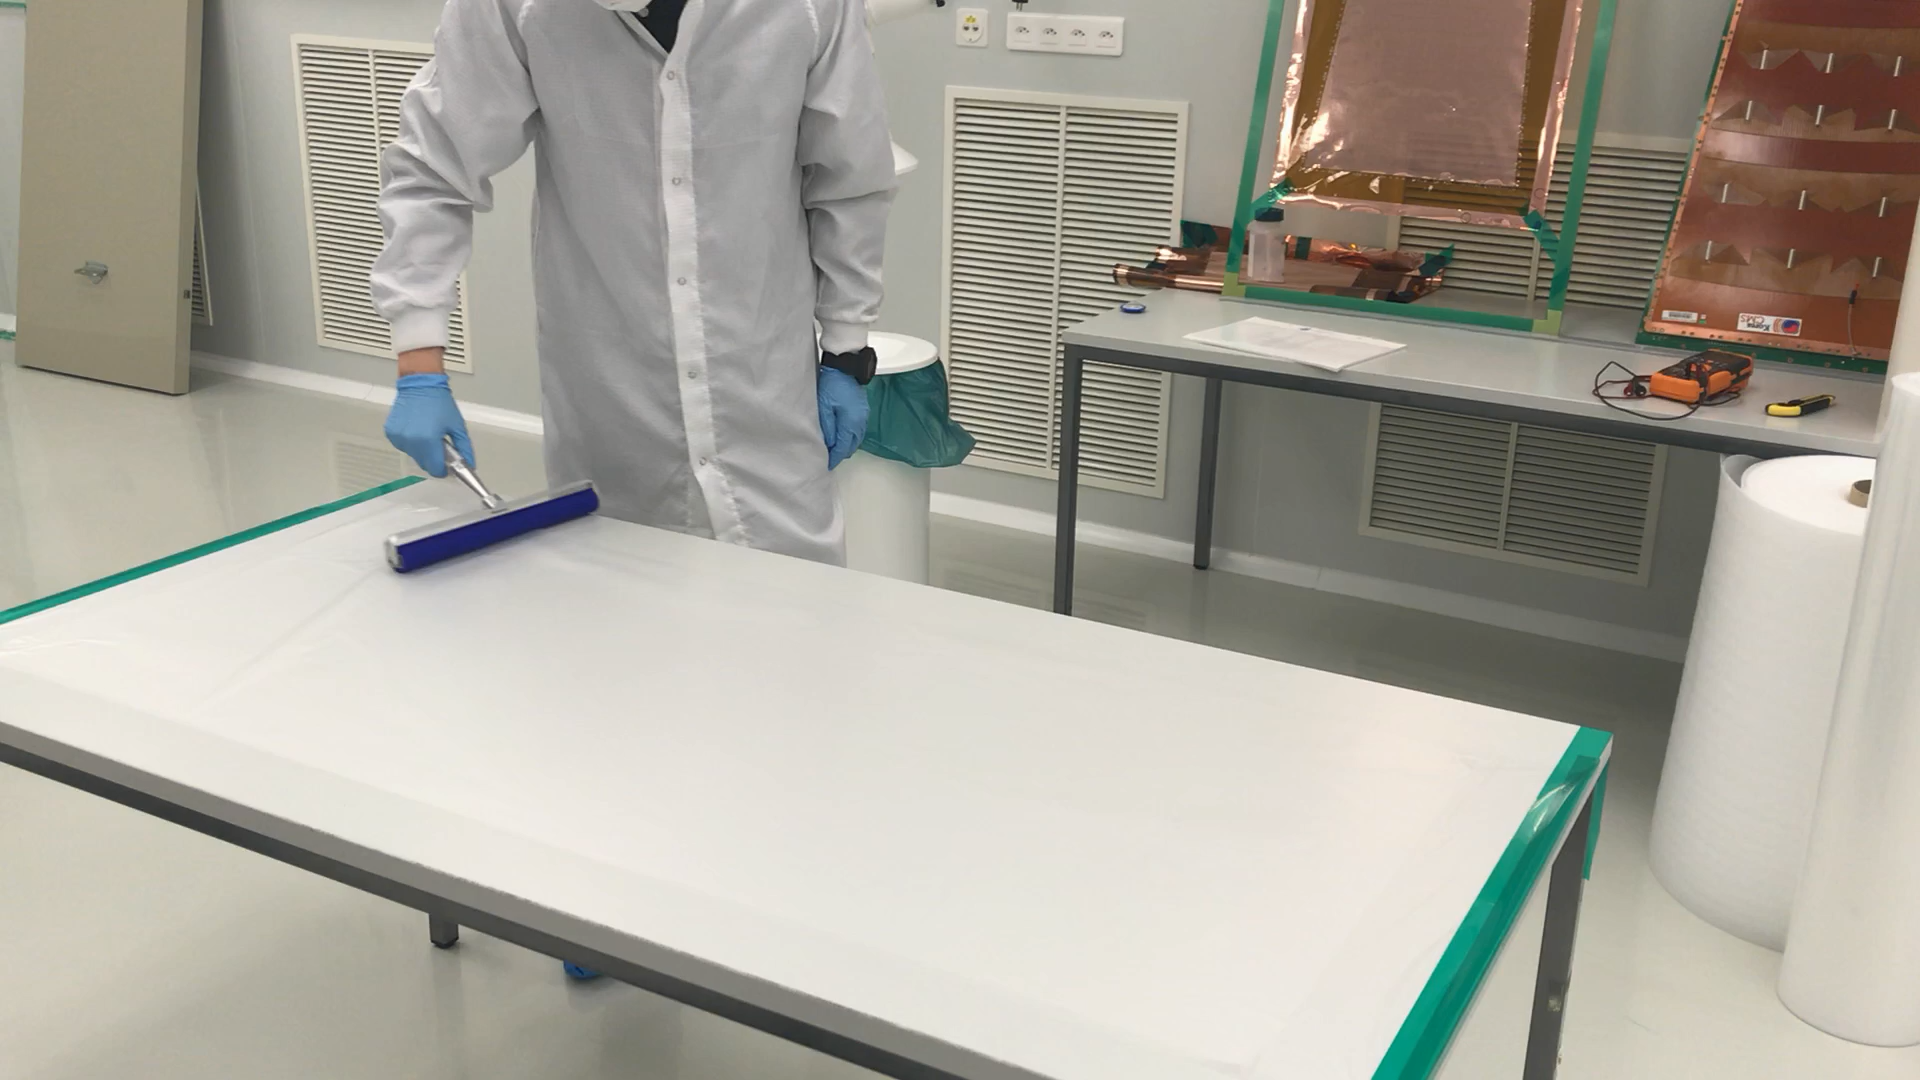
\includegraphics[width=0.40\textwidth]{cleaning_antistatic.png}
  }
  \subfloat{
    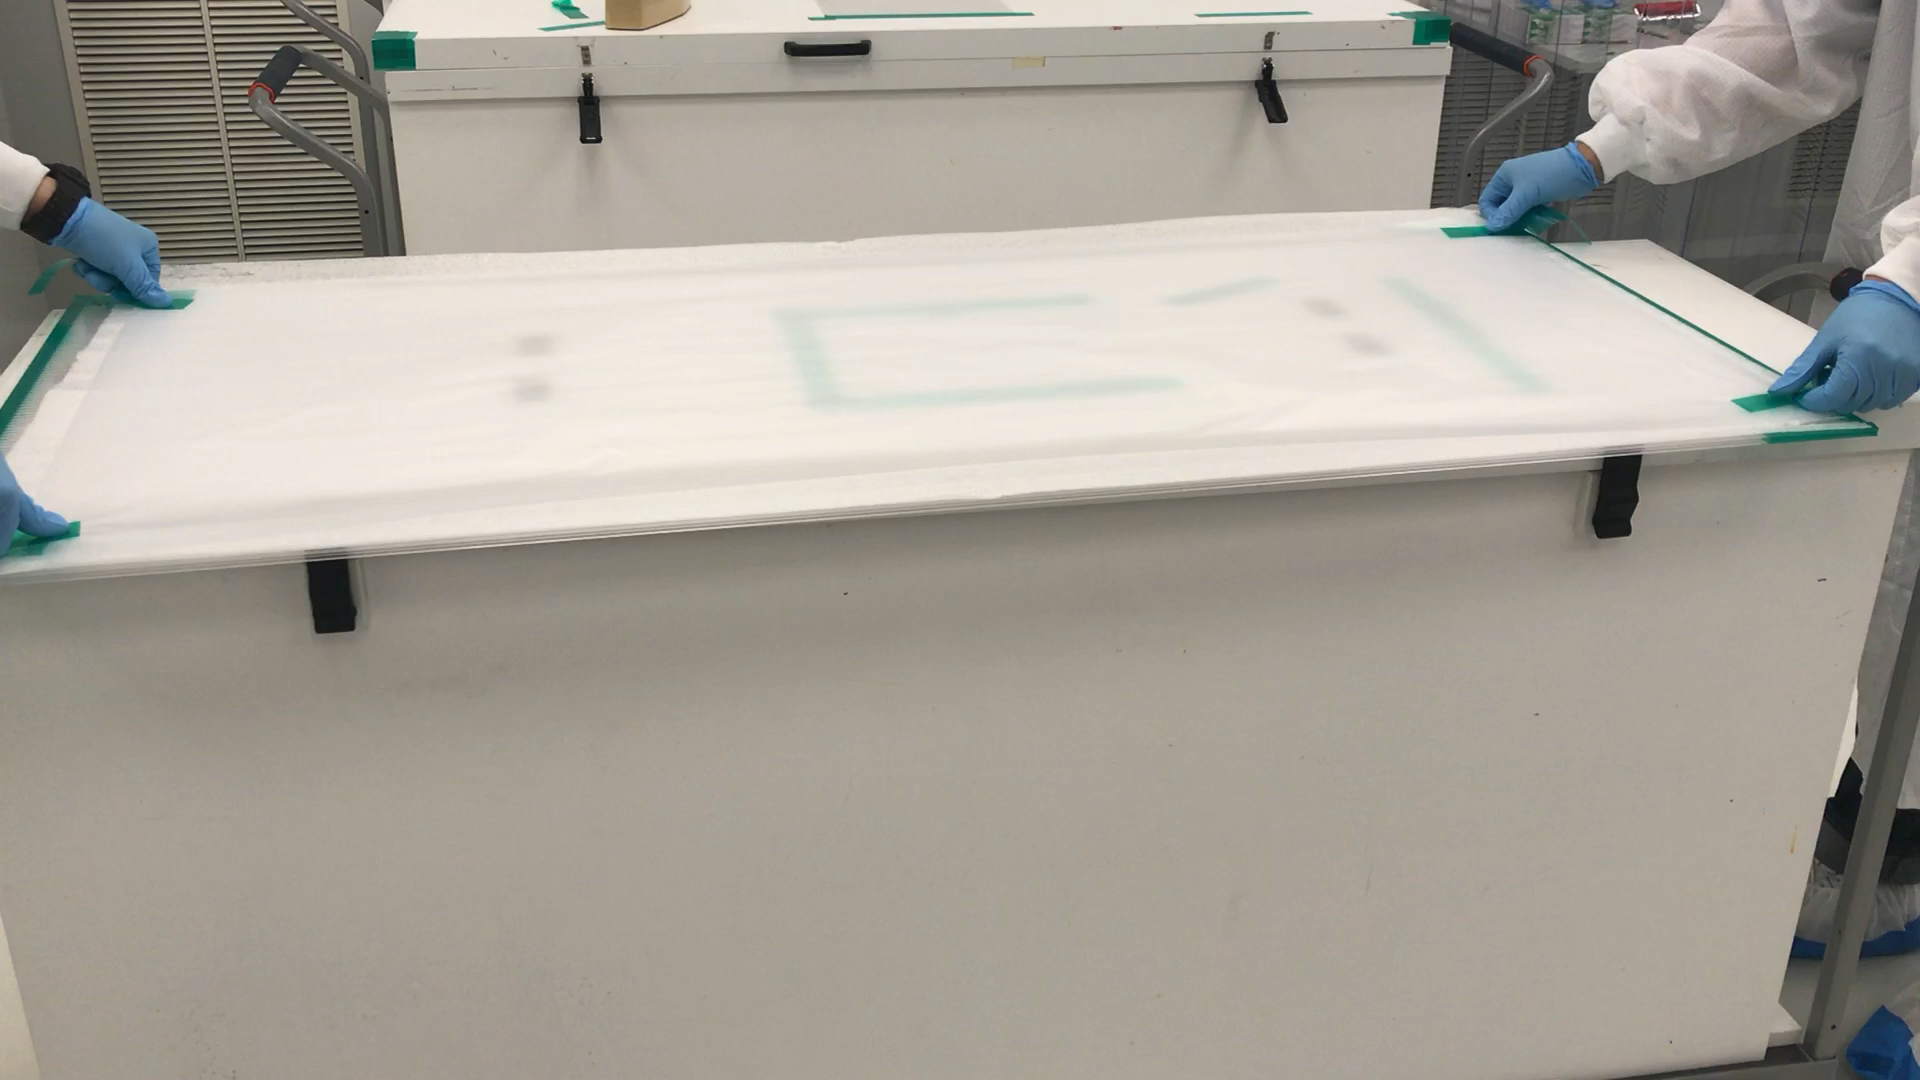
\includegraphics[width=0.40\textwidth]{fixing_antistatic.png}
  }
  \caption[방전 필름의 처리]{왼쪽 : 방전 필름은 DCR 롤러 이용해 양면을 청소한다. 오른쪽 : 방전 필름은 폴리카보네이트 판에 3M PET 테이프로 네 뒤퉁이를 고정한다. 이 때, 구김이 없어야 한다.}
  \label{fig:anti_static}
\end{figure}

\begin{figure}[htb]
  \centering
  \subfloat{
    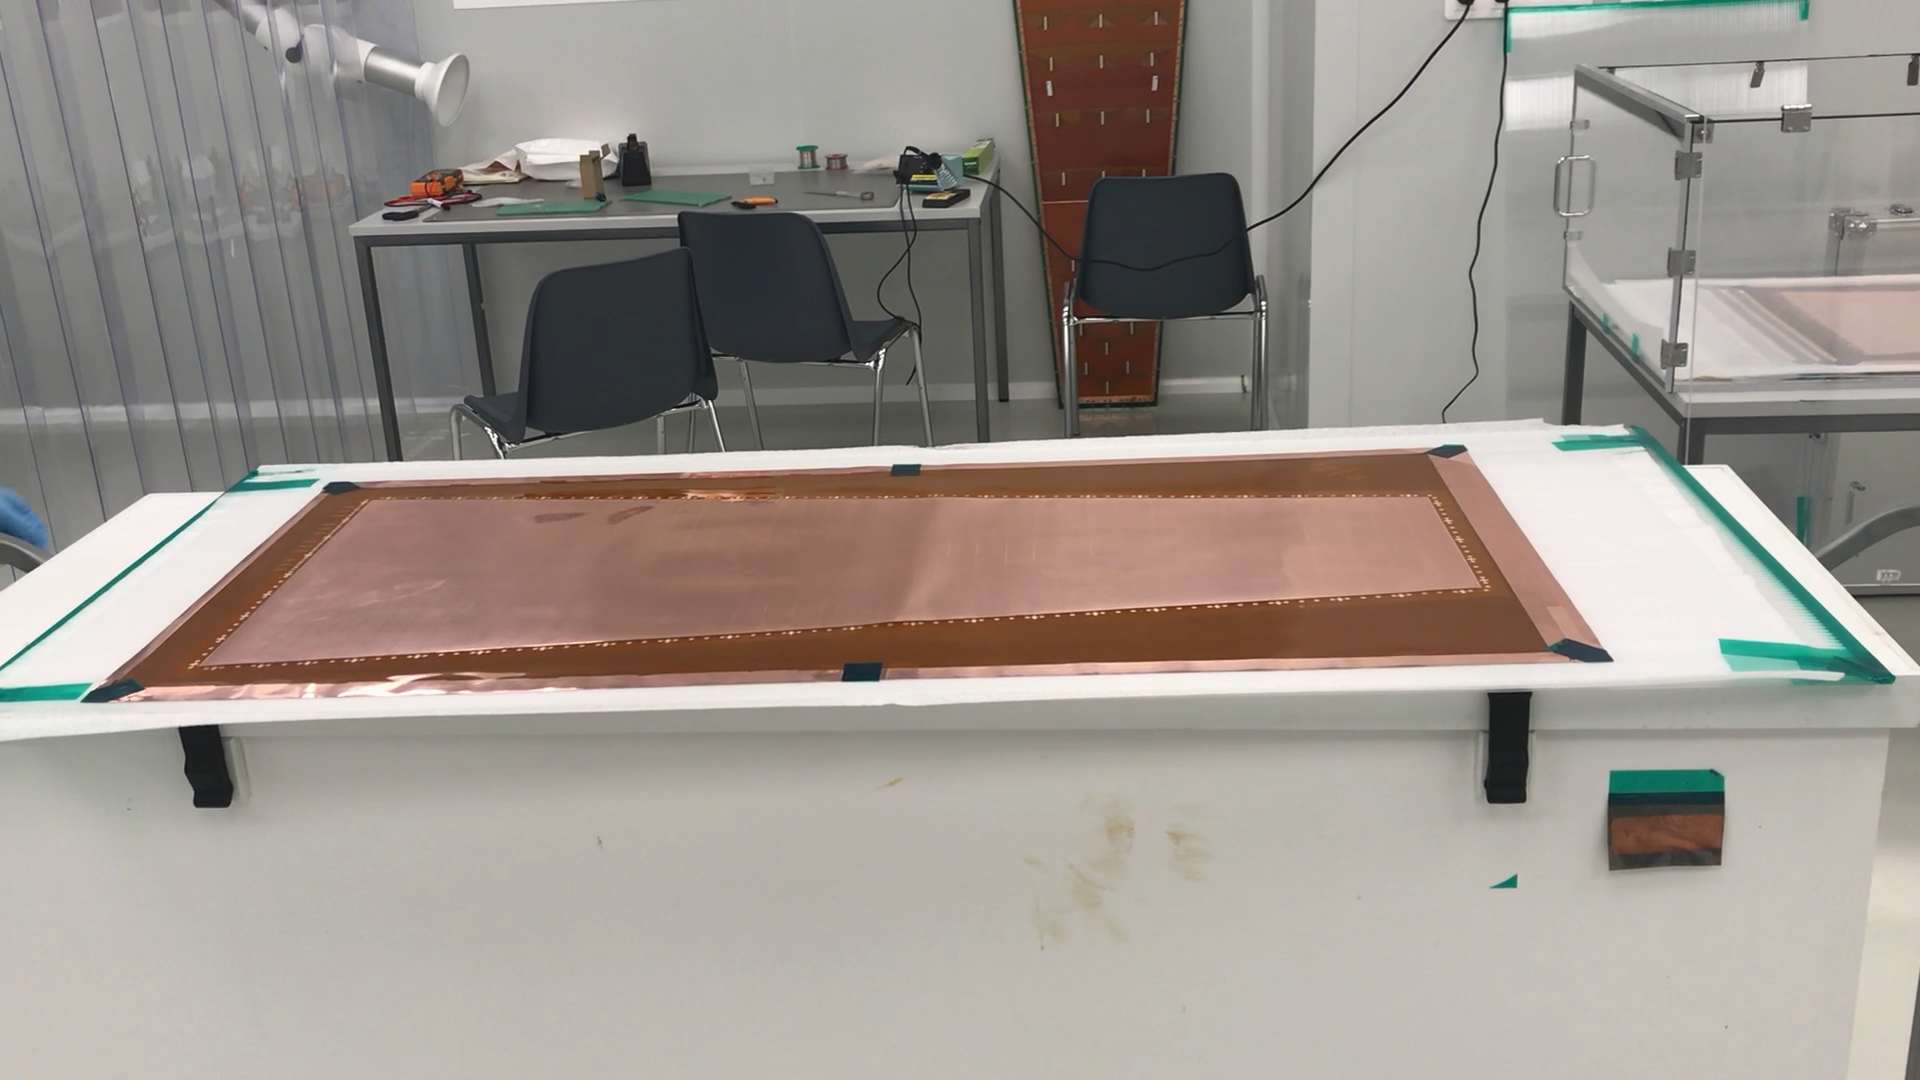
\includegraphics[width=0.40\textwidth]{fixing_foil_0.png}
  }
  \subfloat{
    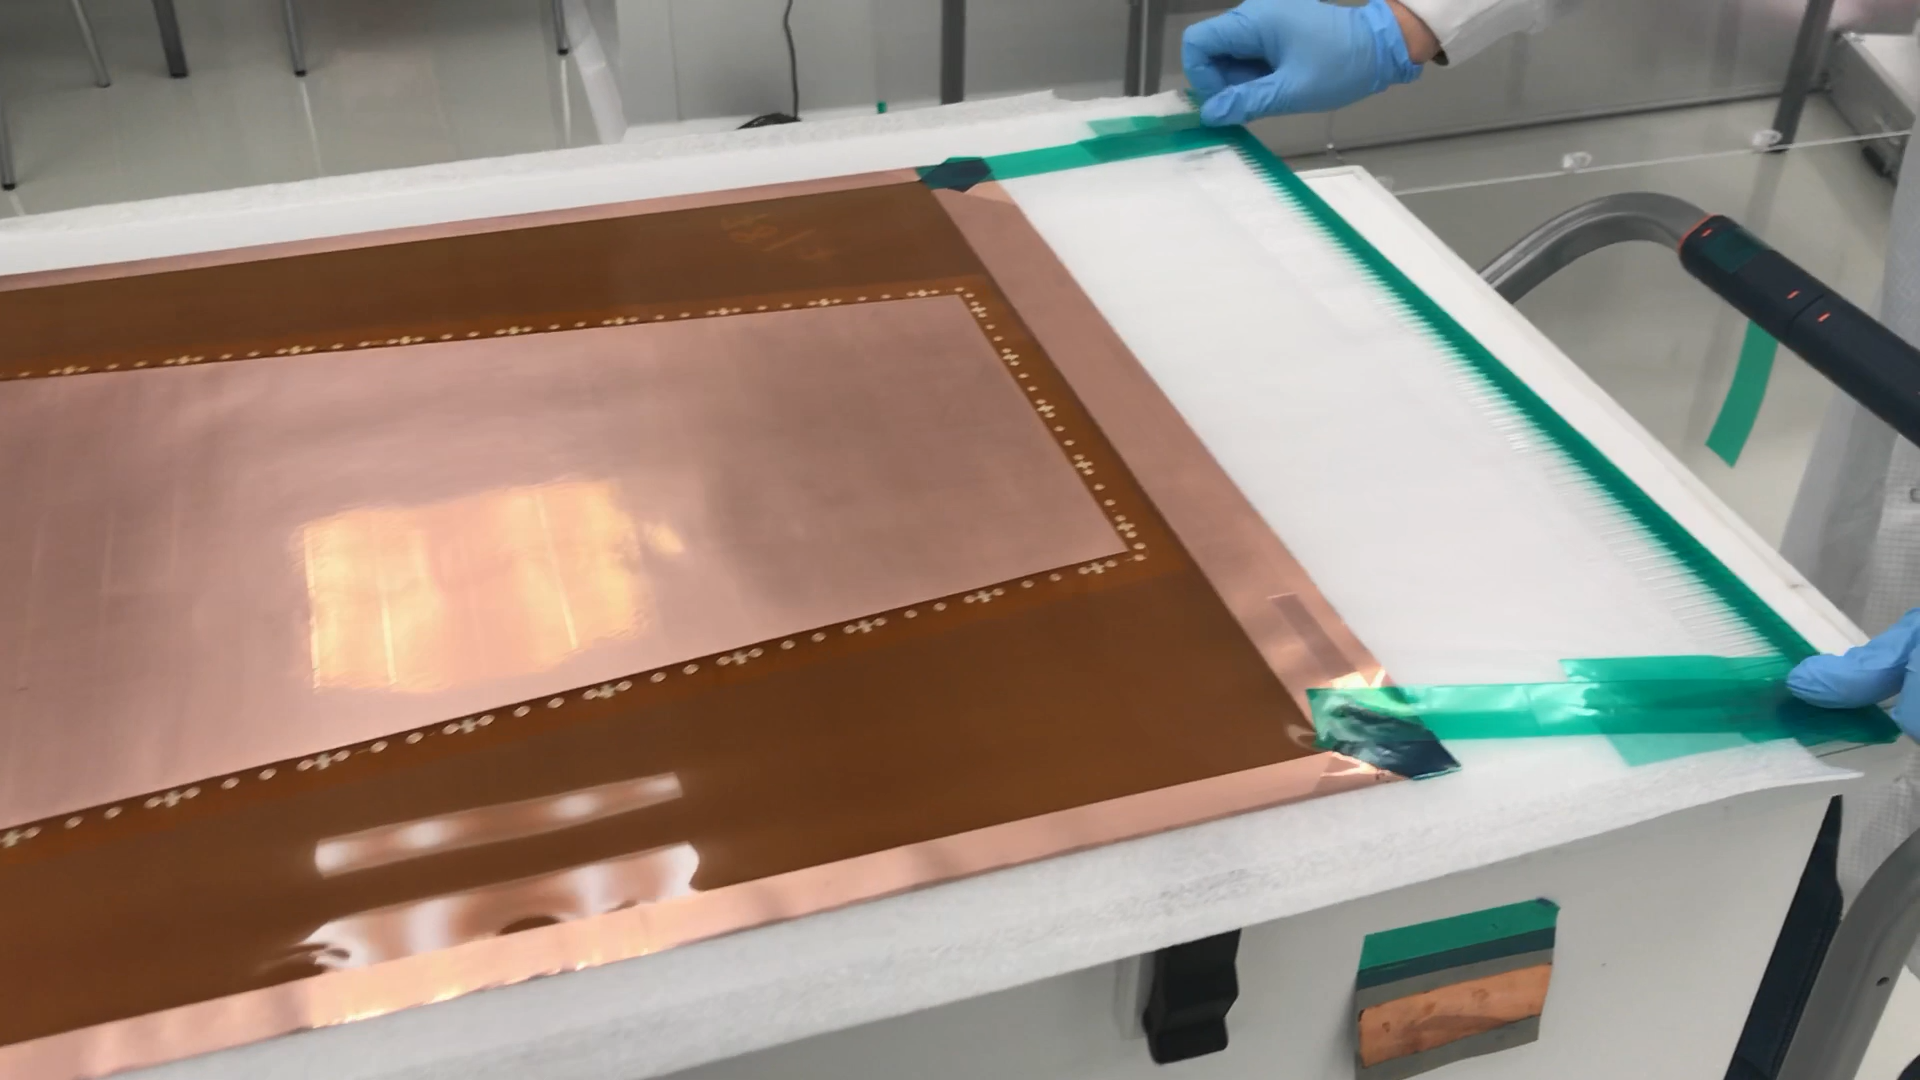
\includegraphics[width=0.40\textwidth]{fixing_foil_1.png}
  }
  \caption[GEM 포일의 고정]{왼쪽 : 포일을 고정하는 폴리카보네이트 판, 폼, 방전 필름의 크기는, GEM 포일의 구겨짐을 방지하기 위해, 포일보다 반드시 커야한다. 오른쪽: GEM 포일은 폴리카보네이트 판에 3M PET 테이프로 네 뒤퉁이를 고정한다.}
  \label{fig:fixing_foil}
\end{figure}


\end{document}

